\documentclass[10pt,a4paper%,twoside,openright,titlepage,fleqn,%
% headinclude,footinclude,BCOR5mm,%
% numbers=noenddot,cleardoublepage=empty,%
tablecaptionabove]{article}

\usepackage{geometry}
\geometry{left=2.5cm,right=2.5cm,top=2.5cm,bottom=2.5cm}
%\usepackage{subfigure}
\usepackage{amsmath,amssymb,amsthm}

%% -----------------设置数学公式字体-------------------------
%% Font style 1
%% \newcommand\ibinom[2]{\genfrac\lbrace\rbrace{0pt}{}{#1}{#2}}
%% \usepackage{bm}

%% Font style 2
%% \newcommand\ibinom[2]{\genfrac\lbrace\rbrace{0pt}{}{#1}{#2}} 
%% \usepackage[boldsans]{ccfonts} 
%% \usepackage{bm} 

%% Font style 3
\newcommand\ibinom[2]{\genfrac\lbrace\rbrace{0pt}{}{#1}{#2}}
\usepackage[euler-digits]{eulervm}
\usepackage{bm}

%% Font style 4
%% \usepackage{fourier}
%% \newcommand\ibinom[2]{\genfrac\lbrace\rbrace{0pt}{}{#1}{#2}}
%% \usepackage{bm}

%% Font style 5
%% \newcommand\ibinom[2]{\genfrac\lbrace\rbrace{0pt}{}{#1}{#2}}
%% \usepackage{mathptmx}
%% \usepackage{bm} 


%% %% Font style 6
%% \newcommand\ibinom[2]{\genfrac\lbrace\rbrace{0pt}{}{#1}{#2}}
%% \usepackage{txfonts}
%% \usepackage{bm}
%% -----------------------------------------------------------

% \usepackage{titlesec} %设置标题
% \usepackage{titletoc}

\usepackage{extarrows}
\usepackage{verbatim,color,xcolor}
\usepackage{pgf}
\usepackage{tikz}
\usetikzlibrary{calc}
\usetikzlibrary{arrows,snakes,backgrounds,shapes,patterns}
\usetikzlibrary{matrix,fit,positioning,decorations.pathmorphing}
%% \usepackage{classicthesis}
\usepackage{CJK}
\usepackage{mathdots}

\usepackage{listings}
\lstset{
  keywordstyle=\color{blue!70},
  frame=single,
  basicstyle=\ttfamily\small,
  commentstyle=\small\color{red},
  breakindent=0pt,
  rulesepcolor=\color{red!20!green!20!blue!20},
  rulecolor=\color{black},
  tabsize=4,
  numbersep=5pt,
  breaklines=true,
  %% backgroundcolor=\color{red!10},
  showspaces=false,
  showtabs=false,
  extendedchars=false,
  escapeinside=``,
  frame=no,
}
\renewcommand{\proofname}{\textbf{证明}}
\renewcommand{\figurename}{\textbf{图}}
\newcommand{\blue}{\textcolor{blue}}
\newcommand{\red}{\textcolor{red}}
\newcommand{\purple}{\textcolor{purple}}
\newcommand{\ds}{\displaystyle}
\newcommand{\cd}{\cdots}
\newcommand{\dd}{\ddots}
\newcommand{\vd}{\vdots}
\newcommand{\id}{\iddots}

\newcommand{\R}{\mathbb R}
\def\nn{{\boldsymbol{n}}}
\def\xx{{\boldsymbol{x}}}
\def\F{{\boldsymbol{F}}}
\def\tf{\ttfamily}


\begin{document}

\begin{CJK}{UTF8}{gkai}
  \renewcommand{\proofname}{\textbf{证明}}
  \renewcommand{\figurename}{\textbf{图}}


  \newtheorem{li}{例}
  \newtheorem{jielun}{结论}
  \newtheorem{dingli}{定理}
  \newtheorem{mingti}{{命题}} 
  \newtheorem{yinli}{{引理}} 
  \newtheorem{tuilun}{{推论}}
  \newtheorem{dingyi}{{定义}} 
  \newtheorem{example}{{例}}
  \newtheorem*{example*}{{例}}
  \newtheorem*{jie}{{解}}
  \newtheorem*{zhengming}{{证明}}
  \newtheorem{zhu}{{注}}
  \newtheorem*{zhu*}{{注}}
  \newtheorem{xingzhi}{{性质}}
  \newtheorem{wenti}{{问题}}
  \newtheorem{rem}{{Remark}}
  \newtheorem{lem}{{Lemma}}
  \pagenumbering{roman}
  \pagestyle{plain}

  \pagenumbering{arabic}

  \title{第一讲、行列式}
  % \author{张晓平}
  % \date{}                                           % Activate to display a given date or no date
  \maketitle

  \section{行列式的定义}
  \subsection{二阶行列式}
  %%%%% 
  \begin{li}
    用消元法求解
    $$
    \left \lbrace
      \begin{array}{l}
        a_{11} x_1 + a_{12} x_2 = b_1, \\[0.2cm]
        a_{21} x_1 + a_{22} x_2 = b_2.
      \end{array}
    \right.
    $$
  \end{li}  
  消去$x_2$得
  $$
  (a_{11}a_{22}-a_{12}a_{21})x_1 = b_1 a_{22} - b_2 a_{12},
  $$
  消去$x_1$得
  $$
  (a_{11}a_{22}-a_{12}a_{21})x_2 = b_2 a_{11} - b_1 a_{11}.
  $$
  若$\boxed{\red{a_{11}a_{22}-a_{12}a_{21}\ne0}}$,则
  $$
  x_1 = \frac{b_1 a_{22} - b_2 a_{12}}{a_{11}a_{22}-a_{12}a_{21}}, \ \
  x_2 = \frac{b_2 a_{11} - b_1 a_{11}}{a_{11}a_{22}-a_{12}a_{21}}.
  $$

  %%%% 
  \begin{dingyi}[二阶行列式]
    由$2^2=4$个数,按下列形式排成2行2列的方形
    $$
    \left|
      \begin{array}{cc}
        a_{11} & a_{12} \\[0.2cm]
        a_{21} & a_{22} 
      \end{array}
    \right|,
    $$
    其被定义成一个数
    $$
    \left|
      \begin{array}{cc}
        a_{11} & a_{12} \\[0.2cm]
        a_{21} & a_{22} 
      \end{array}
    \right| = a_{11}a_{22} - a_{12}a_{21} \equiv D,
    $$
    该数称为由这四个数构成的二阶行列式。
  \end{dingyi}
  %%%% 
  $\red{a_{ij}}$表示行列式的元素。
  $i$为行标,表明该元素位于第$i$行;
  $j$为列标,表明该元素位于第$j$列。

  \begin{figure}[htbp]
    \centering      
    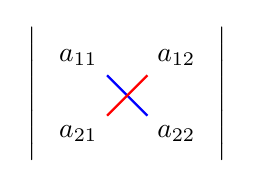
\begin{tikzpicture}
      \matrix (A) [matrix of nodes,ampersand replacement=\&,row sep=15pt,column sep=15pt,left delimiter=|,
      right delimiter=|] {
        $a_{11}$ \& $a_{12}$  \\
        $a_{21}$ \& $a_{22}$  \\
      };
      \draw[blue, thick] (A-1-1.south east) -- (A-2-2.north west);
      \draw[red,  thick] (A-1-2.south west) -- (A-2-1.north east);
    \end{tikzpicture}
    \caption{对角线法则}
  \end{figure}

  %%%%%% 
  
  类似地,
  $$
  \begin{array}{l}
    b_1 a_{22} - b_2 a_{12} = \left|
    \begin{array}{cc}
      b_1 & a_{12} \\
      b_2 & a_{22} 
    \end{array}
            \right|  \equiv D_1\\[0.4cm]
    b_2 a_{11} - b_1 a_{21} = \left|
    \begin{array}{cc}
      a_{11} & b_1 \\
      a_{21} & b_2
    \end{array}
               \right|  \equiv D_2\\
  \end{array}
  $$      
  则上述方程组的解可表示为
  $$
  x_1 = \frac{D_1}{D},\ \
  x_2 = \frac{D_2}{D}.
  $$

  \begin{li}
    求解二元线性方程组
    $$
    \left\{
      \begin{array}{l}
        3x_1 - 2x_2 = 12, \\[0.2cm]
        2x_1 + x_2  = 1.
      \end{array}
    \right.
    $$
  \end{li}
  解:因为
  $$
  \begin{array}{l}
    D = \left|
    \begin{array}{cc}
      3 & -2 \\
      2 & 1 
    \end{array}
          \right| = 7 \ne 0,\\[0.4cm]
    D_1 = \left|
    \begin{array}{cc}
      12 & -2 \\
      1 & 1 
    \end{array}
          \right| = 14 , \\[0.4cm]
    D_2 = \left|
    \begin{array}{cc}
      3 & 12 \\
      2 & 1 
    \end{array}
          \right| = -21,
  \end{array}
  $$
  因此,
  $$
  x_1=\frac{D_1}{D}=2, \ \ x_2 = \frac{D_2}{D} = -3.
  $$

  \subsection{三阶行列式}
  \begin{dingyi}[三阶行列式]
    由$3^2=9$个数组成的3行3列的三阶行列式,则按如下形式定义一个数
    $$
    \begin{aligned}
      D_3 &= 
      \left|
        \begin{array}{ccc}
          a_{11} & a_{12} & a_{13} \\[0.2cm]
          a_{21} & a_{22} & a_{23} \\[0.2cm]
          a_{31} & a_{32} & a_{33} 
        \end{array}
      \right|
      \\
      &=  a_{11}a_{22}a_{33} + a_{12}a_{23}a_{31} + a_{13}a_{21}a_{32}
      - a_{13}a_{22}a_{31} - a_{11}a_{23}a_{32} - a_{12}a_{21}a_{33}
    \end{aligned}
    $$
  \end{dingyi}

  \begin{figure}[htbp]
    \centering
    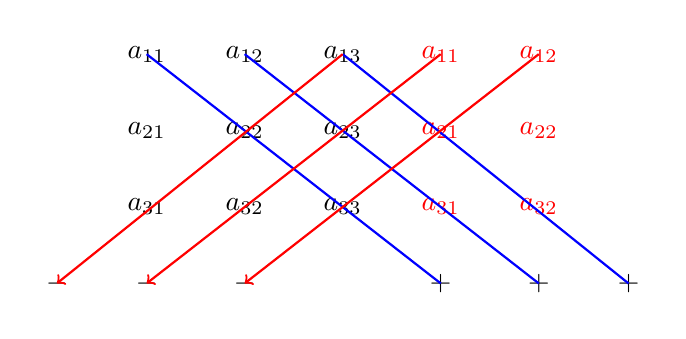
\begin{tikzpicture}               
      \matrix(A) [matrix of math nodes,nodes in empty cells,ampersand replacement=\&,row sep=15pt,column sep=15pt] {
        \&  a_{11} \& a_{12} \& a_{13}  \& \red{a_{11}} \& \red{a_{12}} \&\\
        \&  a_{21} \& a_{22} \& a_{23}  \& \red{a_{21}} \& \red{a_{22}} \&\\
        \&  a_{31} \& a_{32} \& a_{33}  \& \red{a_{31}} \& \red{a_{32}} \&\\
        -   \&    -        \&   -        \&               \&   +         \&   +        \& +\\
      };
      \draw[blue,thick] (A-1-2.center) -- (A-4-5.center);
      \draw[blue,thick] (A-1-3.center)  -- (A-4-6.center);
      \draw[blue,thick] (A-1-4.center) -- (A-4-7.center); 
      \draw[red,thick,->] (A-1-6.center) -- (A-4-3.center);
      \draw[red,thick,->] (A-1-5.center) -- (A-4-2.center);
      \draw[red,thick,->] (A-1-4.center) -- (A-4-1.center); 
    \end{tikzpicture}
    \caption{沙路法}
  \end{figure}

  \begin{li}
    计算
    $$
    D_3 = 
    \left |
      \begin{array}{rrr}
        1  & 2 & -4 \\ 
        -2 & 2 & 1  \\
        -3 & 4 & -2
      \end{array}
    \right|
    $$
  \end{li}
  \begin{jie}
    由沙路法可知,
    $$
    \begin{array}{ll}
      D_3 &=   1\times   2  \times (-2) +   2  \times 1 \times (-3) + (-2) \times 4 \times (-4)\\[0.2cm]
          & - 2\times (-2) \times (-2) - (-4) \times 2 \times (-3) +   1  \times 1 \times   4\\[0.2cm]
          & = -14.
    \end{array}
    $$
  \end{jie}

  \begin{li}
    求方程
    $$
    \left |
      \begin{array}{ccc}
        1  & 1 & 1 \\
        2  & 3 & x  \\
        4  & 9 & x^2
      \end{array}
    \right| = 0
    $$        
  \end{li}
  \begin{jie}
    行列式
    $$ 
    D = 3x^2 + 18 + 4x - 2x^2 - 12 - 9x 
    = x^2 - 5x + 6
    $$
    由此可知$x=2$或$3$。
  \end{jie}


  如果三元一次方程组
  $$
  \begin{array}{c}  
    a_{11}x_1 + a_{12}x_2 + a_{13}x_3 = b_1, \\
    a_{21}x_1 + a_{22}x_2 + a_{23}x_3 = b_2, \\
    a_{31}x_1 + a_{32}x_2 + a_{33}x_3 = b_3,
  \end{array}
  $$
  的系数行列式
  $$
  D = \left|
    \begin{array}{ccc}
      a_{11} & a_{12} & a_{13}\\
      a_{21} & a_{22} & a_{23}\\
      a_{31} & a_{32} & a_{33}
    \end{array}
  \right| \ne 0
  $$
  则用消元法求解可得
  $$
  x_1 = \frac{D_1}{D}, \quad
  x_2 = \frac{D_2}{D}, \quad
  x_3 = \frac{D_3}{D}, \quad
  $$
  其中
  $$
  D_1 = \left|
    \begin{array}{ccc}
      b_1 & a_{12} & a_{13}\\
      b_2 & a_{22} & a_{23}\\
      b_3 & a_{32} & a_{33}
    \end{array}
  \right|, \
  D_2 = \left|
    \begin{array}{ccc}
      a_{11} & b_1 & a_{13}\\
      a_{21} & b_2 & a_{23}\\
      a_{31} & b_3 & a_{33}
    \end{array}
  \right|, \
  D_3= \left|
    \begin{array}{ccc}
      a_{11} & a_{12} & b_1 \\
      a_{21} & a_{22} & b_2 \\
      a_{31} & a_{32} & b_3 
    \end{array}
  \right|.
  $$

  从二、三阶行列式的展开式中可发现:
  $$
  \begin{array}{l}
    D  =  \left|
    \begin{array}{ccc}
      a_{11} & a_{12} & a_{13}\\
      a_{21} & a_{22} & a_{23}\\
      a_{31} & a_{32} & a_{33}
    \end{array}
                        \right| \\[0.6cm]
    = 
    a_{11}a_{22}a_{33}+a_{12}a_{23}a_{31}+a_{13}a_{21}a_{32}
    -a_{13}a_{22}a_{31}-a_{12}a_{21}a_{33}-a_{11}a_{23}a_{32} \\[0.3cm] 
    = 
    a_{11}(a_{22}a_{33}-a_{23}a_{32})-
    a_{12}(a_{21}a_{33}-a_{23}a_{31})+
    a_{13}(a_{21}a_{32}-a_{22}a_{31}) \\[0.3cm] 
    = 
    a_{11} \underbrace{\left| \begin{array}{ccc} a_{22} & a_{33} \\ a_{23} & a_{32} \end{array} \right|}_{M_{11}} -
                                                                             a_{12} \underbrace{\left| \begin{array}{ccc} a_{21} & a_{23} \\ a_{31} & a_{33} \end{array} \right|}_{M_{12}} +
                                                                                                                                                      a_{13} \underbrace{\left| \begin{array}{ccc} a_{21} & a_{22} \\ a_{31} & a_{32} \end{array} \right|}_{M_{13}}
  \end{array}
  $$
  这里,$M_{11},M_{12},M_{13}$分别称为$a_{11},a_{12},a_{13}$的\red{余子式},并称
  $$
  A_{11} = (-1)^{1+1} M_{11}, \quad
  A_{12} = (-1)^{1+2} M_{12}, \quad
  A_{13} = (-1)^{1+3} M_{13}
  $$
  分别称为$a_{11},a_{12},a_{13}$的\red{代数余子式}。 这样,$D$可表示为
  $$
  D= a_{11}A_{11} + a_{11}A_{13} + a_{13}A_{13}.
  $$

  同样地,
  $$
  D = \left| \begin{array}{ccc} a_{11} & a_{12} \\ a_{21} & a_{22} \end{array} \right|
  = a_{11} A_{11} + a_{12} A_{12},
  $$
  其中
  $$
  A_{11} = (-1)^{1+1}|a_{22}| =  a_{22},\quad
  A_{11} = (-1)^{1+2}|a_{21}| = -a_{21}.
  $$
  注意这里的$|a_{22}|,~|a_{21}|$是一阶行列式,而不是绝对值。
  我们把一阶行列式$|a|$定义为$a$。


  \subsection{$n$阶行列式的定义}
  \begin{dingyi}[$n$阶行列式]
    由$n^2$个数$a_{ij}(i,j=1,2,\cdots,n)$组成的$n$阶行列式
    \begin{equation}\label{Dn}
      D = \left|
        \begin{array}{cccc}
          a_{11}  &  a_{12} & \cdots & a_{1n} \\
          a_{21}  &  a_{22} & \cdots & a_{2n} \\
          \vdots & \vdots & \ddots & \vdots\\  
          a_{n1}  &  a_{n2} & \cdots & a_{nn} 
        \end{array}
      \right|
    \end{equation}
    是一个数。
    \begin{itemize}
    \item 当$n=1$时,定义$D=|a_{11}|=a_{11}$; 
    \item 当$n\ge2$时,定义
      \begin{equation}
        D = a_{11} A_{11} + a_{12} A_{12} + \cdots + a_{1n} A_{1n},
      \end{equation}
      其中
      $$A_{1j} = (-1)^{1+j} M_{1j}$$
      而$M_{1j}$是$D$中划去第$1$行第$j$列后,按原顺序排成的$n-1$阶行列式,即
      $$
      M_{1j} =   \left|
        \begin{array}{cccccc}
          a_{21}  & \cdots&  a_{2,j-1}  &  a_{2,j+1}  & \cdots & a_{2n} \\
          a_{31}  & \cdots&  a_{3,j-1}  &  a_{3,j+1}  & \cdots & a_{3n} \\
          \vdots &       &  \vdots &  \vdots &  & \vdots\\  
          a_{n1}  & \cdots&  a_{n,j-1}  &  a_{n,j+1}  & \cdots & a_{nn} 
        \end{array}
      \right| \quad (j = 1,2,\cdots, n),
      $$
      并称$M_{1j}$为$a_{1j}$的余子式,$A_{1j}$为$a_{1j}$的代数余子式.
    \end{itemize}
  \end{dingyi}

  \begin{zhu}
    需注意以下两点:
    \begin{enumerate}
    \item[1]
      在$D$中,$a_{11},a_{22},\cdots,a_{nn}$所在的对角线称为行列式的\red{主对角线},$a_{11},a_{22},\cdots,a_{nn}$称为\red{主对角元}。
    \item[2]
      行列式$D$是由$n^2$个元素构成的$n$次齐次多项式:
      \begin{itemize}
      \item 二阶行列式的展开式有$2!$项;
      \item 三阶行列式的展开式有$3!$项;
      \item $n$阶行列式的展开式有$n!$项,其中每一项都是不同行不同列的$n$个元素的乘积,带正号的项与带负号的项各占一半。
      \end{itemize}      
    \end{enumerate}    
  \end{zhu}
  由行列式的定义可知,一个$n$阶行列式可以展开成$n$个$n$阶行列式之和,即
  $$
  \begin{aligned}
    \left|
      \begin{array}{cccc}
        a_{11}  &  a_{12} & \cdots & a_{1n} \\
        a_{21}  &  a_{22} & \cdots & a_{2n} \\
        \vdots & \vdots & \ddots & \vdots\\  
        a_{n1}  &  a_{n2} & \cdots & a_{nn} 
      \end{array}
    \right| &= 
    \left|
      \begin{array}{cccc}
        a_{11}  &  0 & \cdots & 0 \\
        0  &  a_{22} & \cdots & a_{2n} \\
        \vdots & \vdots & \ddots & \vdots\\  
        0  &  a_{n2} & \cdots & a_{nn} 
      \end{array}
    \right|  + \left|
      \begin{array}{ccccc}
        0  &  a_{12} & 0 & \cdots & 0 \\
        a_{21} & 0  &  a_{23} & \cdots & a_{2n} \\
        \vdots & \vdots & \vdots & \ddots & \vdots\\  
        a_{n1}  & 0&  a_{n3} & \cdots & a_{nn} 
      \end{array}
    \right| \\[0.1in]
    & \quad + \cdots  
    + 
    \left|
      \begin{array}{cccc}
        0 & \cdots & 0 & a_{1n} \\
        a_{21}  &   \cdots & a_{2,n-1} & 0 \\
        \vdots &  \ddots & \vdots & \vdots\\  
        a_{n1}  &   \cdots & a_{n,n-1} & 0
      \end{array}
    \right| 
  \end{aligned}
  $$

  
  \begin{li}
    证明:$n$阶下三角行列式
    $$
    D_n = \left|
      \begin{array}{cccc}
        a_{11}  &  0 & \cdots & 0 \\
        a_{21}  &  a_{22} & \cdots & 0 \\
        \vdots & \vdots & \ddots & \vdots\\  
        a_{n1}  &  a_{n2} & \cdots & a_{nn} 
      \end{array}
    \right| = a_{11} a_{22} \cdots a_{nn}.
    $$  
  \end{li}
  \begin{proof}
    用数学归纳法证明。
    \begin{enumerate}
    \item 当$n=2$时,结论成立。 
    \item 假设结论对$n-1$阶下三角阵成立,则由定义
      $$
      \begin{array}{rcl}
        \left|
        \begin{array}{cccc}
          a_{11}  &  0 & \cdots & 0 \\
          a_{21}  &  a_{22} & \cdots & 0 \\
          \vdots & \vdots & \ddots & \vdots\\  
          a_{n1}  &  a_{n2} & \cdots & a_{nn} 
        \end{array}
                                       \right| &=&  a_{11} \cdot (-1)^{1+1} \left|
                                                   \begin{array}{cccc}
                                                     a_{22}  &  0 & \cdots & 0 \\
                                                     a_{31}  &  a_{33} & \cdots & 0 \\
                                                     \vdots & \vdots & \ddots & \vdots\\  
                                                     a_{n1}  &  a_{n2} & \cdots & a_{nn} 
                                                   \end{array}
                                                                                  \right| \\[0.1in]
                  &=&  a_{11} (a_{22} a_{33} \cdots a_{nn}). \quad \qed        
      \end{array}
      $$    
    \end{enumerate}
    综上所述,结论成立。
  \end{proof}

  同理可证
  $$
  \left|
    \begin{array}{cccc}
      a_{11}  &  0 & \cdots & 0 \\
      0  &  a_{22} & \cdots & 0 \\
      \vdots & \vdots & \ddots & \vdots\\  
      0  &  0 & \cdots & a_{nn} 
    \end{array}
  \right| = a_{11}a_{22}\cdots a_{nn}
  $$

  \begin{li}
    计算$n$阶行列式
    $$
    \left|
      \begin{array}{ccccc}
        0  &  0 & \cdots & 0 & a_n \\
        0  &  0 & \cdots & a_{n-1} & * \\
        \vdots & \vdots & & \vdots & \vdots\\  
        0  &  a_2 & \cdots & * & * \\
        a_1 & * & \cdots & * & *
      \end{array}
    \right| 
    $$
  \end{li}
  \begin{jie}
    由行列式定义,
    $$
    \begin{array}{rcl}
      D_n &=& \left|
              \begin{array}{ccccc}
                0  &  0 & \cdots & 0 & a_n \\
                0  &  0 & \cdots & a_{n-1} & * \\
                \vdots & \vdots & & \vdots & \vdots\\  
                0  &  a_2 & \cdots & * & * \\
                a_1 & * & \cdots & * & *
              \end{array}
                                       \right| =   (-1)^{1+n} a_n \left|
                                       \begin{array}{cccc}
                                         0  &  0 & \cdots &   a_{n-1} \\
                                         \vdots & \vdots &  & \vdots\\  
                                         0  &  a_2 & \cdots  & * \\
                                         a_1 & * & \cdots  & *
                                       \end{array} 
                                                             \right| \\
          &=&  (-1)^{n-1} a_n D_{n-1}.      
    \end{array}
    $$
    同理递推,
    $$
    \begin{array}{rcl}
      D_n & =& (-1)^{n-1} a_n D_{n-1}  = (-1)^{n-1} a_n (-1)^{n-2} a_{n-1} D_{n-2} \\[0.1in]
          && \cdots\cdots \\[0.2cm]
          &=&   (-1)^{(n-1)+(n-2)+\cdots+2+1} a_n a_{n-1} \cdots a_2 a_1 \\[0.1in]
          &=&  (-1)^{\frac{n(n-1)}{2}} a_n a_{n-1} \cdots a_2 a_1.
    \end{array}
    $$
    例如,
    $$
    D_2 = -a_1a_2, \quad
    D_3 = -a_1a_2a_3, \quad
    D_4 = a_1a_2a_3a_4, \quad
    D_5 = a_1a_2a_3a_4a_5.
    $$
  \end{jie}



  \section{行列式的性质}

  \begin{xingzhi}
    互换行列式的行与列,值不变,即
    \begin{equation}
      \left|
        \begin{array}{cccc}
          a_{11}  &  a_{12} & \cdots & a_{1n} \\
          a_{21}  &  a_{22} & \cdots & a_{2n} \\
          \vdots & \vdots & \ddots & \vdots\\  
          a_{n1}  &  a_{n2} & \cdots & a_{nn} 
        \end{array}
      \right|
      =
      \left|
        \begin{array}{cccc}
          a_{11}  &  a_{21} & \cdots & a_{n1} \\
          a_{12}  &  a_{22} & \cdots & a_{n2} \\
          \vdots & \vdots & \ddots & \vdots\\  
          a_{1n}  &  a_{2n} & \cdots & a_{nn} 
        \end{array}
      \right|
    \end{equation}
  \end{xingzhi}
  \begin{proof}
    将等式两端的行列式分别记为$D$和$D^\prime$,对阶数$n$用归纳法。
    \begin{enumerate}
    \item 当$n=2$时,$D=D^\prime$显然成立。 
    \item 假设结论对于阶数小于$n$的行列式都成立,以下考虑阶数为$n$的情况。由定义可知,
      $$
      \begin{array}{c}
        D = a_{11} A_{11}+a_{12}A_{12}+\cdots+a_{1n}A_{1n}, \\[0.1in]
        D^\prime = a_{11} A^\prime_{11}+a_{21}A^\prime_{21}+\cdots+a_{n1}A^\prime_{n1}
      \end{array}
      $$
      显然,$A_{11}=A^\prime_{11}$。
      于是
      $$
      \begin{aligned}
        D^\prime =&
        a_{11} A_{11}+(-1)^{1+2}a_{21}
        \left|
          \begin{array}{cccc}
            a_{12} & a_{32} & \cdots & a_{n2} \\
            a_{13} & a_{33} & \cdots & a_{n3} \\
            \vdots & \vdots & & \vdots \\
            a_{1n} & a_{3n} & \cdots & a_{nn} \\
          \end{array}
        \right|  + (-1)^{1+3}a_{31}
        \left|
          \begin{array}{ccccc}
            a_{12} & a_{22} & a_{42} & \cdots & a_{n2} \\
            a_{13} & a_{23} & a_{43} & \cdots & a_{n3} \\
            \vdots & \vdots & \vdots & & \vdots \\
            a_{1n} & a_{2n} & a_{4n} & \cdots & a_{nn} \\
          \end{array}
        \right|  \\
        & + \cdots + (-1)^{1+n} a_{n1} \left|
          \begin{array}{cccc}
            a_{12} & a_{22} & \cdots & a_{n-1,2} \\
            a_{13} & a_{23} & \cdots & a_{n-1,3} \\
            \vdots & \vdots & & \vdots \\
            a_{1n} & a_{2n} & \cdots & a_{n-1,n} \\
          \end{array}
        \right|
      \end{aligned}
      $$
      对上式中的$n-1$个行列式按第一行展开,并将含$a_{12}$的项进行合并,可得
      $$
      \begin{aligned}
        & (-1)^{1+2}a_{21} a_{12}
        \left|
          \begin{array}{ccc}       
            a_{33} & \cdots & a_{n3} \\
            \vdots  & & \vdots \\
            a_{3n} & \cdots & a_{nn} \\
          \end{array}
        \right| 
        + (-1)^{1+3}a_{31} a_{12}
        \left|
          \begin{array}{cccc}
            a_{23}  & a_{43} & \cdots & a_{n3} \\
            \vdots & \vdots & & \vdots \\
            a_{2n}  & a_{4n} & \cdots & a_{nn} \\
          \end{array}
        \right|  \\
        & \hspace{2in} + \cdots +(-1)^{1+n} a_{n1} a_{12}
        \left|
          \begin{array}{ccc}
            a_{23} & \cdots & a_{n-1,3} \\
            \vdots & & \vdots \\
            a_{2n} & \cdots & a_{n-1,n} \\
          \end{array}
        \right|\\
        = &   (-1)^{1+2} a_{12} \left(
          (-1)^{1+1} a_{21} 
          \left|
            \begin{array}{ccc}       
              a_{33} & \cdots & a_{n3} \\
              \vdots  & & \vdots \\
              a_{3n} & \cdots & a_{nn} \\
            \end{array}
          \right|    
          + (-1)^{1+2}a_{31} 
          \left|
            \begin{array}{cccc}
              a_{23}  & a_{43} & \cdots & a_{n3} \\
              \vdots & \vdots & & \vdots \\
              a_{2n}  & a_{4n} & \cdots & a_{nn} \\
            \end{array}
          \right|\right.\\
        &  \hspace{2in} \left. + \cdots + (-1)^{1+n-1} a_{n1}
          \left|
            \begin{array}{ccc}
              a_{23} & \cdots & a_{n-1,3} \\
              \vdots & & \vdots \\
              a_{2,n} & \cdots & a_{n-1,n} \\
            \end{array}
          \right|
        \right)\\
        % =  (-1)^{1+2} a_{12} \left(      
        %   \left|
        %     \begin{array}{cccc}       
        %       a_{21} & 0 & \cdots & 0 \\
        %       0 & a_{33} & \cdots & a_{n3} \\
        %       0 & \vdots  & & \vdots \\
        %       0 & a_{3n} & \cdots & a_{nn} \\
        %     \end{array}
        %   \right|  
        %   + 
        %   \left|
        %     \begin{array}{ccccc}
        %       0 & a_{31} & 0 & \cdots & 0 \\
        %       a_{23}  & 0 & a_{43} & \cdots & a_{n3} \\
        %       \vdots & 0 & \vdots & & \vdots \\
        %       a_{2n}  & 0 & a_{4n} & \cdots & a_{nn} \\
        %     \end{array}
        %   \right|  \right.\\
        % + \cdots + \left. 
        %   \left|
        %     \begin{array}{cccc}
        %       0 & \cdots & 0 & a_{n-1} \\
        %       a_{23} & \cdots & a_{n-1,3} & 0 \\
        %       \vdots & & \vdots & 0\\
        %       a_{2,n3} & \cdots & a_{n-1,n} & 0 \\
        %     \end{array}
        %   \right|
        % \right)\\
        = &(-1)^{1+2} a_{12}
        \left|
          \begin{array}{cccc}
            a_{21} & a_{31} & \cdots & a_{n1} \\
            a_{23} & a_{33} & \cdots & a_{n3} \\
            \vdots & \vdots & & \vdots \\
            a_{2n} & a_{3n} & \cdots & a_{nn}        
          \end{array}
        \right| (-1)^{1+2}a_{12} M_{12}^\prime  = a_{12} A_{12}^\prime = a_{12} A_{12}. 
      \end{aligned}
      $$
      同理,含$a_{13}$的项合并后其值等于$a_{13}A_{13}$,$\cdots$,
      含$a_{1n}$的项合并后其值等于$a_{1n}A_{1n}$. 因此,$D=D^\prime$.
    \end{enumerate}

  \end{proof}
  \begin{zhu}
    有了这个性质,行列式对行成立的性质都适用于列。
  \end{zhu}
  
  \begin{xingzhi}
    行列式对任一行按下式展开,其值相等,即
    $$
    D = a_{i1} A_{i1} + a_{i2} A_{i2} + \cdots + a_{in}A_{in} = \sum_{j=1}^n a_{ij} A_{ij}, \quad
    i = 1, 2, \cdots, n,
    $$
    其中
    $$
    A_{ij} = (-1)^{i+j} M_{ij}
    $$
    而$M_{ij}$为$a_{ij}$的余子式,$A_{ij}$为$a_{ij}$的代数余子式.
  \end{xingzhi}
  \begin{proof}
    对$n$用归纳法证明。
    \begin{enumerate}
    \item 当$n=2$时,结论显然成立。
    \item 假设结论对阶数$\le n-1$的行列式成立,以下考虑阶数为$n$的情况。
      $$
      \begin{aligned}
        D = &  (-1)^{1+1} a_{11} \left|
          \begin{array}{cccc}
            a_{22}  & a_{23}   & \cdots & a_{2n}\\
            \vdots  & \vdots & & \vdots \\
            a_{i2}  & a_{i3}   & \cdots & a_{in}\\
            \vdots & \vdots  & & \vdots \\
            a_{n2}  & a_{n3}   & \cdots & a_{nn}\\
          \end{array}
        \right| + (-1)^{1+2} a_{12} \left|
          \begin{array}{cccc}
            a_{21}  & a_{23}  & \cdots & a_{2n}\\
            \vdots & \vdots & & \vdots \\
            a_{i1}  & a_{i3}  & \cdots & a_{in}\\
            \vdots & \vdots & & \vdots \\
            a_{n1}  & a_{n3}  & \cdots & a_{nn}\\
          \end{array}
        \right|\\
        & + (-1)^{1+3} a_{13} \left|
          \begin{array}{ccccc}
            a_{21}  & a_{22} & a_{24}  & \cdots & a_{2n}\\
            \vdots & \vdots & \vdots & & \vdots \\
            a_{i1}  & a_{i2} & a_{24}  & \cdots & a_{in}\\
            \vdots & \vdots & \vdots & & \vdots \\
            a_{n1}  & a_{n2}  & a_{n4} & \cdots & a_{nn}\\
          \end{array}
        \right|
        + \cdots  
        + (-1)^{1+n} a_{1n} \left|
          \begin{array}{cccc}
            a_{21}  & a_{22}   & \cdots & a_{2,n-1}\\
            \vdots  & \vdots & & \vdots \\
            a_{i1}  & a_{i2}   & \cdots & a_{i,n-1}\\
            \vdots & \vdots  & & \vdots \\
            a_{n1}  & a_{n2}   & \cdots & a_{n,n-1}\\
          \end{array}
        \right|
      \end{aligned}
      $$
      由归纳假设,按第$i$行展开后合并含$a_{i1}$的项得,
      $$
      \begin{aligned}
        (-1)^{(i-1)+1}a_{i1} \left ( (-1)^{1+2} a_{12}  \left|
            \begin{array}{cccc}
              a_{23}  & a_{24}  & \cdots & a_{2n}\\
              \vdots & \vdots & & \vdots \\
              a_{i-1,3}  & a_{i-1,4}  & \cdots & a_{i-1,n}\\
              a_{i+1,3}  & a_{i+1,4}  & \cdots & a_{i+1,n}\\
              \vdots & \vdots & & \vdots \\
              a_{n,3}  & a_{n,4}  & \cdots & a_{nn}
            \end{array}
          \right| + (-1)^{1+3} a_{13}   \left|
            \begin{array}{cccc}
              a_{22} & a_{24}  & \cdots & a_{2n}\\
              \vdots & \vdots & & \vdots \\
              a_{i-1,2} & a_{i-1,4}  & \cdots & a_{i-1,n}\\
              a_{i+1,2} & a_{i+1,4}  & \cdots & a_{i+1,n}\\
              \vdots & \vdots & & \vdots \\
              a_{n2}  & a_{n4} & \cdots & a_{nn}
            \end{array}
          \right|
        \right.\\
        \hspace{2in} \left. + \cdots  +  (-1)^{1+n} a_{1n}  \left|
            \begin{array}{ccc}
              a_{22}   & \cdots & a_{2,n-1}\\
              \vdots & & \vdots \\
              a_{i-1,2}   & \cdots & a_{i-1,n-1}\\
              a_{i+1,2}   & \cdots & a_{i+1,n-1}\\
              \vdots  & & \vdots \\
              a_{n2}   & \cdots & a_{n,n-1}
            \end{array}
          \right| \right) 
      \end{aligned}
      $$
      即
      $$
      (-1)^{i+1}a_{i1} \left|
        \begin{array}{cccc}
          a_{12} & a_{13} & \cdots & a_{1n} \\
          a_{22} & a_{23} & \cdots & a_{2n}\\
          \vdots & \vdots & & \vdots \\
          a_{i-1,2} & a_{i-1,3}   & \cdots & a_{i-1,n}\\    
          a_{i-1,2} & a_{i-1,3}   & \cdots & a_{i-1,n}\\
          \vdots & \vdots & & \vdots \\
          a_{n2}  & a_{n3} & \cdots & a_{nn}
        \end{array}
      \right| = (-1)^{i+1}a_{i1} M_{i1} = a_{i1} A_{i1}.
      $$
      同理可证,含$a_{i2}$的项合并后其值为$a_{i2}A_{i2}$,$\cdots$,含$a_{in}$的项合并后其值为$a_{in}A_{in}$.  
    \end{enumerate}

  \end{proof}


  \begin{xingzhi}[线性性质]
    \begin{itemize}
    \item[1] 行列式的某一行(列)中所有的元素都乘以同一个数$k$,等于用数$k$乘以此行列式,即
      \begin{equation}\label{xz3-1}
        \left|
          \begin{array}{ccccc}
            a_{11}  & a_{12} & \cdots & a_{1n} \\
            \vdots & \vdots     &        & \vdots \\
            ka_{i1}  & ka_{i2} & \cdots & ka_{in} \\
            \vdots & \vdots     &        & \vdots \\
            a_{n1}  & a_{n2} & \cdots & a_{nn}
          \end{array}
        \right| = k
        \left|
          \begin{array}{ccccc}
            a_{11}  & a_{12} & \cdots & a_{1n} \\
            \vdots & \vdots     &        & \vdots \\
            a_{i1}  & a_{i2} & \cdots & a_{in} \\
            \vdots & \vdots     &        & \vdots \\
            a_{n1}  & a_{n2} & \cdots & a_{nn}
          \end{array}
        \right|
      \end{equation}
    \item[2] 若行列式的某一行(列)的元素都是两数之和,如       \begin{equation}\label{xz3-2}
        \begin{array}{rcl}
          \left|
          \begin{array}{ccccc}
            a_{11} & \cdots & a_{1j}+b_{1j} & \cdots & a_{1n} \\
            a_{21} & \cdots & a_{2j}+b_{2j} & \cdots & a_{2n} \\
            \vdots&        & \vdots      &        & \vdots \\
            a_{n1} & \cdots & a_{nj}+b_{nj} & \cdots & a_{nn}
          \end{array}
                                                       \right| & = & \left|
                                                                     \begin{array}{ccccc}
                                                                       a_{11} & \cdots & a_{1j} & \cdots & a_{1n} \\
                                                                       a_{21} & \cdots & a_{2j} & \cdots & a_{2n} \\
                                                                       \vdots&        & \vdots      &        & \vdots \\
                                                                       a_{n1} & \cdots & a_{nj} & \cdots & a_{nn}
                                                                     \end{array}
                                                                                                           \right| +
                                                                                                           \left|
                                                                                                           \begin{array}{ccccc}
                                                                                                             a_{11} & \cdots & b_{1j} & \cdots & a_{1n} \\
                                                                                                             a_{21} & \cdots & b_{2j} & \cdots & a_{2n} \\
                                                                                                             \vdots&        & \vdots      &        & \vdots \\
                                                                                                             a_{n1} & \cdots & b_{nj} & \cdots & a_{nn}
                                                                                                           \end{array}
                                                                                                                                                 \right|          
        \end{array}
      \end{equation}
    \end{itemize}
  \end{xingzhi}
  \begin{zhu}一些记号:
    \begin{itemize}
    \item $r_i\times k$($c_i\times k$):第$i$行(列)乘以$k$
    \item $r_i\div k$($c_i\div k$):第$i$行(列)提取公因子$k$
    \end{itemize}
  \end{zhu}
  \begin{dingyi}[反对称行列式]
    如果行列式$D=|a_{ij}|_{n}$的元素$a_{ij}=-a_{ji}(i,j=1,2,\cdots,n)$,就称$D$是反对称行列式(其中$a_{ii}=-a_{ii}\Rightarrow a_{ii}=0,i=1,2,\cdots,n$).
  \end{dingyi}
  \begin{li}
    证明:奇数阶反对称行列式的值为$0$.
  \end{li}
  \begin{proof}
    $$
    \begin{aligned}
      D &= \left|
        \begin{array}{cccc}
          0 & a_{12} & \cd & a_{1n} \\
          -a_{12} & 0 & \cd & a_{2n} \\
          \vd & \vd & \dd & \vd \\
          -a_{1n} & -a_{2n} & \cd & 0
        \end{array}
      \right|
      \xlongequal[]{\text{性质1}}   \left|
        \begin{array}{cccc}
          0 & -a_{12} & \cd & -a_{1n} \\
          a_{12} & 0 & \cd & -a_{2n} \\
          \vd & \vd & \dd & \vd \\
          a_{1n} & a_{2n} & \cd & 0
        \end{array}
      \right| \\
      &  \xlongequal[\text{将每行提取公因子$-1$}]{\text{性质3-1}} 
      (-1)^n \left|
        \begin{array}{cccc}
          0 & a_{12} & \cd & a_{1n} \\
          -a_{12} & 0 & \cd & a_{2n} \\
          \vd & \vd & \dd & \vd \\
          -a_{1n} & -a_{2n} & \cd & 0
        \end{array}
      \right| = (-1)^n D.
    \end{aligned}  
    $$
    由于$n$为奇数,故$D=-D$,从而$D=0$.
  \end{proof}

  \begin{tuilun}
    若行列式的某行元素全为0,其值为0.
  \end{tuilun}

  \begin{li}
    $$
    \left|
      \begin{array}{ccc}
        1 & 2 & 3\\
        0 & 0 & 0\\
        2 & 5 & 1
      \end{array}
    \right| = 0.
    $$
  \end{li}
  
  \begin{xingzhi}
    若行列式有两行(列)完全相同,其值为$0$.
  \end{xingzhi}
  \begin{proof}
    不妨设$D$的第$i$和$j$行元素全部相等,即对
    $$
    D = \left|
      \begin{array}{cccc}
        a_{11}  &  a_{12} & \cdots & a_{1n} \\
        \vdots & \vdots &  & \vdots\\  
        a_{i1}  &  a_{i2} & \cdots & a_{in} \\
        \vdots & \vdots &  & \vdots\\  
        a_{j1}  &  a_{j2} & \cdots & a_{jn} \\
        \vdots & \vdots &  & \vdots\\  
        a_{n1}  &  a_{n2} & \cdots & a_{nn} 
      \end{array}
    \right|,
    $$
    有$a_{il}=a_{jl}(i\ne j, l=1,2,\cdots,n)$.
    对阶数$n$用数学归纳法。
    \begin{itemize}
    \item 当$n=2$时,结论显然成立。
    \item 假设结论对阶数为$n-1$的行列式成立,在$n$阶的情况下,对第$k(k\ne i, j)$行展开,有
      $$
      D = a_{k1} A_{k1} + a_{k2} A_{k2} + \cdots + a_{kn} A_{kn}. 
      $$ 
      注意到余子式$M_{kl}(l=1,2,\cdots,n)$是$n-1$阶行列式,且其中有两行元素相同,故
      $$
      A_{kl} = (-1)^{k+l} M_{kl} = 0\quad (l=1,2,\cdots,n),
      $$
      从而$D=0$.
    \end{itemize}
  \end{proof}
  \begin{li}
    $$
    \left|
      \begin{array}{ccc}
        1 & 2 & 3\\
        1 & 2 & 3\\
        2 & 3 & 4
      \end{array}
    \right| = 0.
    $$
  \end{li}

  \begin{tuilun}
    若行列式中有两行(列)元素成比例,则行列式的值为$0$.
  \end{tuilun}
  \begin{li}
    $$
    \left|
      \begin{array}{ccc}
        2 & 0 & -2\\
        1 & 0 & -1\\
        2 & 3 & 4
      \end{array}
    \right| =2 \left|
      \begin{array}{ccc}
        1 & 0 & -1\\
        1 & 0 & -1\\
        2 & 3 & 4
      \end{array}
    \right| = 0.
    $$
  \end{li}

  
  \begin{xingzhi}
    把行列式的某一行(列)的各元素乘以同一个数然后加到另一行(列)对应的元素上去,行列式的值不变。
  \end{xingzhi}
  \begin{proof}
    将数$k$乘以第$j$行加到第$i$行,有
    $$
    \begin{array}{ll}
      & \left|
        \begin{array}{cccc}
          a_{11} & a_{12} & \cdots & a_{1n}\\
          \vdots & \vdots &  & \vdots \\
          a_{i1}+k a_{j1} & a_{i2}+k a_{j2} & \cdots & a_{in}+k a_{jn}\\
          \vdots & \vdots &  & \vdots \\
          a_{j1} & a_{j2} & \cdots & a_{jn}\\
          \vdots & \vdots &  & \vdots \\
          a_{n1} & a_{n2} & \cdots & a_{nn}
        \end{array}
                                     \right|
    \end{array}
    $$
    $$
    \begin{array}{ll}
      \xlongequal[]{\text{性质3-2}} & 
                                      \left|
                                      \begin{array}{cccc}
                                        a_{11} & a_{12} & \cdots & a_{1n}\\
                                        \vdots & \vdots &  & \vdots \\
                                        a_{i1} & a_{i2} & \cdots & a_{in}\\
                                        \vdots & \vdots &  & \vdots \\
                                        a_{j1} & a_{j2} & \cdots & a_{jn}\\
                                        \vdots & \vdots &  & \vdots \\
                                        a_{n1} & a_{n2} & \cdots & a_{nn}
                                      \end{array}
                                                                   \right| +
                                                                   \left|
                                                                   \begin{array}{cccc}
                                                                     a_{11} & a_{12} & \cdots & a_{1n}\\
                                                                     \vdots & \vdots &  & \vdots \\
                                                                     k a_{j1} & k a_{j2} & \cdots & k a_{jn}\\
                                                                     \vdots & \vdots &  & \vdots \\
                                                                     a_{j1} & a_{j2} & \cdots & a_{jn}\\
                                                                     \vdots & \vdots &  & \vdots \\
                                                                     a_{n1} & a_{n2} & \cdots & a_{nn}
                                                                   \end{array}
                                                                                                \right|\\[0.2in]
      \xlongequal[]{\text{推论2}}  & 
                                     \left|
                                     \begin{array}{cccc}
                                       a_{11} & a_{12} & \cdots & a_{1n}\\
                                       \vdots & \vdots &  & \vdots \\
                                       a_{i1} & a_{i2} & \cdots & a_{in}\\
                                       \vdots & \vdots &  & \vdots \\
                                       a_{j1} & a_{j2} & \cdots & a_{jn}\\
                                       \vdots & \vdots &  & \vdots \\
                                       a_{n1} & a_{n2} & \cdots & a_{nn}
                                     \end{array}
                                                                  \right|
    \end{array}
    $$
  \end{proof}
  \begin{zhu}一些记号:
    \begin{itemize}
    \item $r_i + r_j\times k$:将第$j$行乘以$k$加到第$i$行;
    \item $c_i + c_j\times k$:将第$j$列乘以$k$加到第$i$列。 
    \end{itemize}

  \end{zhu}


  \begin{xingzhi}
    互换行列式的两行(列),行列式变号。
  \end{xingzhi}
  \begin{proof}
    $$
    \begin{aligned}
      D &= \left|
        \begin{array}{cccc}
          a_{11} & a_{12} & \cdots & a_{1n}\\
          \vdots & \vdots &  & \vdots \\
          a_{i1} & a_{i2} & \cdots & a_{in}\\
          \vdots & \vdots &  & \vdots \\
          a_{j1} & a_{j2} & \cdots & a_{jn}\\
          \vdots & \vdots &  & \vdots \\
          a_{n1} & a_{n2} & \cdots & a_{nn}
        \end{array}
      \right| \xlongequal[r_i+r_j]{\text{性质5}} 
      \left|
        \begin{array}{cccc}
          a_{11} & a_{12} & \cdots & a_{1n}\\
          \vdots & \vdots &  & \vdots \\
          a_{i1}+a_{j1} & a_{i2}+a_{j2} & \cdots & a_{in}+a_{jn}\\
          \vdots & \vdots &  & \vdots \\
          a_{j1} & a_{j2} & \cdots & a_{jn}\\
          \vdots & \vdots &  & \vdots \\
          a_{n1} & a_{n2} & \cdots & a_{nn}
        \end{array}
      \right|\\
      &\xlongequal[r_j-r_i]{\text{性质5}} 
      \left|
        \begin{array}{cccc}
          a_{11} & a_{12} & \cdots & a_{1n}\\
          \vdots & \vdots &  & \vdots \\
          a_{i1}+a_{j1} & a_{i2}+a_{j2} & \cdots & a_{in}+a_{jn}\\
          \vdots & \vdots &  & \vdots \\
          -a_{i1} & -a_{i2} & \cdots & -a_{in}\\
          \vdots & \vdots &  & \vdots \\
          a_{n1} & a_{n2} & \cdots & a_{nn}
        \end{array}
      \right|
      \xlongequal[r_i+r_j]{\text{性质5}} 
      \left|
        \begin{array}{cccc}
          a_{11} & a_{12} & \cdots & a_{1n}\\
          \vdots & \vdots &  & \vdots \\
          a_{j1} & a_{j2} & \cdots & a_{jn}\\
          \vdots & \vdots &  & \vdots \\
          -a_{i1} & -a_{i2} & \cdots & -a_{in}\\
          \vdots & \vdots &  & \vdots \\
          a_{n1} & a_{n2} & \cdots & a_{nn}
        \end{array}
      \right| \xlongequal[]{\text{性质3-1}} - D.
    \end{aligned}
    $$
  \end{proof}

  \begin{zhu}一些记号:
    \begin{itemize}
    \item $r_i \leftrightarrow r_j $:互换第$i,j$行 \\[0.1in]
    \item $c_i \leftrightarrow c_j $:互换第$i,j$列
    \end{itemize}
  \end{zhu}
  \begin{li}
    $$
    \begin{array}{rcl}
      \left|
      \begin{array}{ccc}
        1 & 2  \\
        3 & 4  \\
      \end{array}
      \right|
          &\xlongequal[]{r_1\leftrightarrow r_2}&
                                                  -\left|
                                                  \begin{array}{ccc}
                                                    3 & 4 \\
                                                    1 & 2 
                                                  \end{array}
                                                        \right|    \\[0.2in]
      \left|
      \begin{array}{ccc}
        1 & 2  \\
        3 & 4  
      \end{array}
            \right|
          &\xlongequal[]{c_1\leftrightarrow c_2}&
                                                  -\left|
                                                  \begin{array}{ccc}
                                                    2 & 1  \\
                                                    4 & 3  
                                                  \end{array}
                                                        \right|    
    \end{array}
    $$    
  \end{li}

  \begin{xingzhi}
    行列式某一行的元素乘以另一行对应元素的代数余子式之和等于$0$,即
    $$
    \sum_{k=1}^n a_{ik} A_{jk}  = 0 \quad (i\ne j).
    $$
  \end{xingzhi}
  \begin{proof}
    由性质2,对$D$的第$j$行展开得
    $$
    \left|
      \begin{array}{cccc}
        a_{11} & a_{12} & \cdots & a_{1n}\\
        \vdots & \vdots &  & \vdots \\
        a_{i1} & a_{i2} & \cdots & a_{in}\\
        \vdots & \vdots &  & \vdots \\
        a_{j1} & a_{j2} & \cdots & a_{jn}\\
        \vdots & \vdots &  & \vdots \\
        a_{n1} & a_{n2} & \cdots & a_{nn}
      \end{array}
    \right|   =  a_{j1} A_{j1} + a_{j2} A_{j2} + \cdots + a_{jn} A_{jn}
    $$
    因此,将$D$中第$j$行的元素$a_{j1},a_{j2},\cdots,a_{jn}$换成$a_{i1},a_{i2},\cdots,a_{in}$后所得的行列式,
    其展开式就是$\sum_{k=1}^na_{ik}A_{jk}$,即
    $$
    \left|
      \begin{array}{cccc}
        a_{11}  &  a_{12} & \cdots & a_{1n} \\
        \vdots & \vdots &  & \vdots\\  
        a_{i1}  &  a_{i2} & \cdots & a_{in} \\
        \vdots & \vdots &  & \vdots\\  
        a_{i1}  &  a_{i2} & \cdots & a_{in} \\
        \vdots & \vdots &  & \vdots\\  
        a_{n1}  &  a_{n2} & \cdots & a_{nn} 
      \end{array}
    \right|
    \xlongequal[]{\text{性质4}}  0.
    $$  
  \end{proof}

  \begin{jielun}
    \begin{itemize}
    \item 对行列式$D$按行展开,有
      $$
      \sum_{k=1} a_{ik} A_{jk} = \delta_{ij} D,
      $$
      其中$\delta_{ij}$为克罗内克(Kronecker)记号,表示为
      $$
      \delta_{ij} = \left\{
        \begin{array}{ll}
          1 & i=j,\\
          0 & i\ne j.
        \end{array}
      \right.
      $$
    \item 对行列式$D$按列展开,有
      $$
      \sum_{k=1} a_{ki} A_{kj} = \delta_{ij} D,
      $$
    \end{itemize}
  \end{jielun}

  \section{行列式的计算}
  \begin{li}
    计算
    $$
    D = \left|
      \begin{array}{rrrr}
        3   &  1  &  -1  &  2 \\
        -5  &  1  &   3  & -4 \\
        2   &  0  &   1  & -1 \\
        1   & -5  &   3  &  -3 
      \end{array}
    \right|
    $$
  \end{li}
  \begin{jie}
    $$
    \begin{array}{ll}
      D&  \xlongequal[c_4+c_3]{c_1-2c_3}  \left|
         \begin{array}{rrrr}
           5  & 1 & -1 & 1  \\
           -11 & 1 &  3 & -1 \\
           0 & 0 &  1 & 0 \\
           -5 & -5 & 3 & 0 
         \end{array}
                         \right|\\[0.8cm]
       & = (-1)^{3+3} \left| 
         \begin{array}{rrr}
           5 & 1 & 1\\
           -11 & 1 & -1 \\
           -5 & -5 & 0
         \end{array}
                     \right| 
                     \xlongequal{r_2+r_1}
                     \left|
                     \begin{array}{rrr}
                       5 & 1 & 1\\
                       -6 & 2 & 0 \\
                       -5 & -5 & 0
                     \end{array}
                                 \right|\\[0.8cm]
       &  = (-1)^{1+3} \left|
         \begin{array}{rr}
           -6 &  2\\
           -5 & -5
         \end{array}
                \right| = 40.
    \end{array}
    $$    
  \end{jie}

  \begin{li}
    计算
    $$
    D = \left |
      \begin{array}{cccc}
        a &    b &       c &           d  \\
        a &  a+b &   a+b+c &     a+b+c+d  \\
        a & 2a+b & 3a+2b+c &  4a+3b+2c+d  \\
        a & 3a+b & 6a+3b+c & 10a+6b+3c+d   
      \end{array}
    \right|
    $$
  \end{li}
  \begin{jie}
    $$
    \begin{array}{ll}
      D &  \ds \xlongequal[r_2-r_1]{r_4-r_3\atop r_3-r_2}
          \left |
          \begin{array}{cccc}
            a &    b &     c &         d  \\
            0 &    a &   a+b &     a+b+c  \\
            0 &    a &  2a+b &   3a+2b+c  \\
            0 &    a &  3a+b &   6a+3b+c   
          \end{array}\right| \xlongequal[r_3-r_2]{r_4-r_3}\left |
                               \begin{array}{cccc}
                                 a &    b &     c &         d  \\
                                 0 &    a &   a+b &     a+b+c  \\
                                 0 &    0 &     a &      2a+b  \\
                                 0 &    0 &     a &      3a+b   
                               \end{array}
                                                    \right|
      \\[1.0cm]
        &  \ds \xlongequal{r_4-r_3} \left |
          \begin{array}{cccc}
            a &    b &     c &         d  \\
            0 &    a &   a+b &     a+b+c  \\
            0 &    0 &     a &      2a+b  \\
            0 &    0 &     0 &         a   
          \end{array}
                               \right| = a^4.      
    \end{array}
    $$
  \end{jie}

  \begin{li}
    计算
    $$
    D = \left |
      \begin{array}{cccccc}
        1 &  2 &  3 & \cd &  n-1 & n\\
        2 &  3 &  4 & \cd &   n  & 1\\
        3 &  4 &  5 & \cd &   1  & 2\\
        \vd& \vd& \vd&     & \vd  & \vd \\
        n &  1 &  2 & \cd & n-2  & n-1
      \end{array}
    \right|
    $$
  \end{li}
  \begin{jie}
    $$
    \begin{aligned}
      D_n &   
      \xlongequal[i=n,\cdots,2]{r_i-r_{i-1}} 
      \left|
        \begin{array}{cccccc}
          1   &  2 &  3 & \cd &  n-1 & n\\
          1   &  1 &  1 & \cd &   1  & 1-n \\
          1   &  1 &  1 & \cd &  1-n  & 1\\
          \vd & \vd & \vd&     & \vd  & \vd \\
          1   & 1-n &  1 & \cd &   1   & 1
        \end{array}
      \right|\\
      &  
      \xlongequal[i=2,\cdots,n]{c_i-c_1} 
      \left|
        \begin{array}{cccccc}
          1   &  1 &  2 & \cd &  n-2 & n-1\\
          1   &  0 &  0 & \cd &   0  & -n \\
          1   &  0 &  0 & \cd &  -n  & 0\\
          \vd & \vd & \vd&     & \vd  & \vd \\
          1   & -n &  0 & \cd &   0   & 0
        \end{array}
      \right|\\
      &   \xlongequal[i=2,\cd,n]{c_i\div n} n^{n-1} 
      \left|
        \begin{array}{cccccc}
          1   &  \frac 1n & \frac 2n & \cd &  \frac{n-2}n & \frac{n-1}n\\
          1   &  0 &  0 & \cd &   0  & -1 \\
          1   &  0 &  0 & \cd &  -1  & 0\\
          \vd & \vd & \vd&     & \vd  & \vd \\
          1   & -1 &  0 & \cd &   0   & 0
        \end{array}
      \right|\\
      &  \xlongequal{c_1+c_2+\cd+c_n} 
      n^{n-1} \left|
        \begin{array}{cccccc}
          1+\sum_{i-1}^{n-1}\frac in   &  \frac 1n & \frac 2n & \cd &  \frac{n-2}n & \frac{n-1}n\\
          0   &  0 &  0 & \cd &   0  & -1 \\
          0   &  0 &  0 & \cd &  -1  & 0\\
          \vd & \vd & \vd&     & \vd  & \vd \\
          0   & -1 &  0 & \cd &   0   & 0
        \end{array}       
      \right|\\
      &  = n^{n-1} \left[ 1 + \frac 1n \frac {n(n-1)}2\right] 
      (-1)^{\frac{(n-1)(n-2)}2}(-1)^{n-1} = (-1)^{\frac{(n-1)n}2} \frac{n+1}2 n^{n-1}.
    \end{aligned}
    $$
  \end{jie}


  \begin{li}
    计算行列式
    $$
    D_{20} = \left|
      \begin{array}{rrrrrrr}
        1   & 2    & 3    & \cd  & 18    & 19    &  20 \\ 
        2   & 1    & 2    & \cd  & 17    & 18    &  19 \\
        3   & 2    & 1    & \cd  & 16    & 17    &  18 \\
        \vd & \vd  & \vd  & \cd  & \vd   & \vd   &  \vd \\
        20  & 19   & 18   & \cd  & 3     & 2     &  1
      \end{array}
    \right|
    $$    
  \end{li}
  \begin{jie}
    $$
    \begin{array}{ll}
      D_{20} &   \xlongequal[i=19,\cd,1]{c_{i+1}-c_i} 
               \left|
               \begin{array}{rrrrrrr}
                 1   & 1    & 1    & \cd  & 1    & 1    &  1 \\ 
                 2   & -1   & 1    & \cd  & 1    & 1    &  1 \\
                 3   & -1   & -1   & \cd  & 1    & 1    &  1 \\
                 \vd & \vd  & \vd  & \cd  & \vd  & \vd  &  \vd \\
                 % 19  & -1   & -1   & \cd  & -1   & -1   &  1 \\
                 20  & -1   & -1   & \cd  & -1   & -1   &  -1
               \end{array}
                                                          \right| \\[0.5cm]
             & \xlongequal[i=2,\cd,20]{r_i+r_1} 
               \left|
               \begin{array}{rrrrrrr}
                 1   & 1    & 1    & \cd  & 1    & 1    &  1 \\ 
                 3   & 0    & 2    & \cd  & 2    & 2    &  2 \\
                 4   & 0    & 0    & \cd  & 2    & 2    &  2 \\
                 \vd & \vd  & \vd  & \cd  & \vd  & \vd  &  \vd \\
                 % 20  & 0    & 0    & \cd  & 0    & 0    &  2\\
                 21  & 0    & 0    & \cd  & 0    & 0    &  0
               \end{array}
                                                          \right|
                                                          = 21 \times (-1)^{20+1} \times 2^{18} = -21 \times 2^{18}.
    \end{array}
    $$

  \end{jie}


  \begin{li}
    计算元素为$a_{ij}=|i-j|$的$n$阶行列式。
  \end{li}
  \begin{jie}
    $$
    \begin{aligned}
      D_{n} &  =   \left|
        \begin{array}{rrrrrrr}
          0   & 1   & 2    & \cd & n-2  & n-1 \\ 
          1   & 0   & 1    & \cd & n-3  & n-2 \\
          %% 2   & 1   & 0    & \cd & n-4  & n-3 \\
          \vd & \vd & \vd  &     & \vd  & \vd \\
          n-2 & n-3 & n-4  & \cd & 0     & 1 \\
          n-1 & n-2 & n-3  & \cd & 1  & 0 
        \end{array}
      \right| \\
      &   \xlongequal[i=n-1,\cd,1]{c_{i+1}-c_i}   
      \left|
        \begin{array}{rrrrrrr}
          0   & 1   & 1    & \cd & 1  & 1 \\ 
          1   & -1  & 1    & \cd & 1  & 1 \\
          %% 2   & -1  & -1   & \cd & 1  & 1 \\
          \vd & \vd & \vd  &     & \vd & \vd \\
          n-2 & -1  & -1   & \cd & -1 & 1 \\
          n-1 & -1  & -1   & \cd & -1 & -1 
        \end{array}
      \right| \\
      & \xlongequal[i=2,\cd,n]{r_{i}+r_1}  
      \left|
        \begin{array}{rrrrrrr}
          0   & 1   & 1   & \cd & 1   & 1   \\ 
          1   & 0   & 2   & \cd & 2   & 2   \\
          \vd & \vd & \vd &     & \vd & \vd \\
          n-2 & 0   & 0  & \cd  & 0   & 2 \\
          n-1 & 0   & 0  & \cd  & 0   & 0 
        \end{array}
      \right| = (-1)^{n-1}(n-1)2^{n-2}.
    \end{aligned}
    $$
  \end{jie}


  \begin{li}
    计算
    $$
    D= \left|
      \begin{array}{ccccc}
        1 &  2  & 3   &\cd & n   \\
        2 &  2  & 0   &\cd & 0  \\
        3 &  0  & 3   &\cd & 0  \\
        \vd & \vd  \vd  &    & \\
        n &  0  & 0   &\cd & n
      \end{array}
    \right|
    $$
  \end{li}
  \begin{jie}
    $$
    \begin{aligned}
      D & \xlongequal[i=2,\cd,n]{r_1-r_i} & 
      \left|
        \begin{array}{ccccc}
          1-\sum_{i=2}^n i &  0  & 0   &\cd & 0   \\
          2 &  2  & 0   &\cd & 0  \\
          3 &  0  & 3   &\cd & 0  \\
          \vd & \vd & \vd  &    &\vd  \\
          n &  0  & 0   &\cd & n
        \end{array}
      \right|
      =  (1-\sum_{i=2}^n i) \cdot 2 \cdot 3 \cdot \cd \cdot n
      =  \left[2-\frac{(n+1)n}2\right] n!
    \end{aligned}
    $$
  \end{jie}

  如何计算“爪形”行列式
%   \begin{center}
%     \begin{tikzpicture}
%       \matrix(A) [matrix of math nodes,nodes in empty cells,ampersand replacement=\&,left delimiter=|,right delimiter=|] {
%         a_{11} \& a_{12} \& a_{13} \& \cd \& a_{1n} \\
%         a_{21} \& a_{22} \& 0     \& \cd \&  0    \\
%         a_{31} \&  0    \& a_{33} \& \cd \&  0    \\
%         \vd  \&  \vd  \&  \vd  \&     \&  \vd  \\
%         a_{n1} \&  0    \& 0 \& \cd \& a_{nn} \\
%       };
%       \draw[red] (A-1-1.center) -- (A-1-5.center) (A-1-1.center) -- (A-5-1.center) (A-1-1.center) -- (A-5-}5.center);
%   \end{tikzpicture}
% \end{center}
其解法固定,即从第二行开始,每行依次乘一个系数然后加到第一行,使得第一行除第一个元素外都为零,从而得到一个下三角行列式。请自行验证以下行列式(假定$a_i \ne 0$)
$$
D_{n+1} = 
\left|
  \begin{array}{ccccc}
    a_0 &  1  & 1   &\cd & 1   \\
    1   & a_1 & 0   &\cd & 0  \\
    1   & 0   & a_2 &\cd & 0  \\
    \vd & \vd  \vd  &    & \\
    1   & 0   & 0   &\cd & a_n
  \end{array}
\right|  = (a_0 - \sum_{i=1}^n \frac1{a_i}) a_1 a_2 \cd a_n.
$$

类似的方式还可用于求解如下形式的“爪型行列式”
% \begin{figure}[htbp]
%   \centering
%   \subfigure[]{
%     \begin{tikzpicture}[scale=2]
%       \matrix(B) [matrix of math nodes,nodes in empty cells,ampersand replacement=\&,left delimiter=|,right delimiter=|] {
%         \&  \& \\
%         \&  \& \\
%         \&  \& \\ 
%       };
%       \draw[red] (B-1-3.north east) -- (B-1-1.north west) 
%       (B-1-3.north east) -- (B-3-1.south west) 
%       (B-1-3.north east) -- (B-3-3.south east);
%     \end{tikzpicture}
%   }
%   \subfigure[]{
%     \begin{tikzpicture}[scale=2]
%       \matrix(B) [matrix of math nodes,nodes in empty cells,ampersand replacement=\&,left delimiter=|,right delimiter=|] {
%         \&  \& \\
%         \&  \& \\
%         \&  \& \\
%       };
%       \draw[red]
%       (B-3-1.south west) -- (B-1-1.north west) 
%       (B-3-1.south west) -- (B-1-3.north east) 
%       (B-3-1.south west) -- (B-3-3.south east);
%     \end{tikzpicture}
%   }
%   \subfigure[]{
%     \begin{tikzpicture}[scale=2]
%       \matrix(B) [matrix of math nodes,nodes in empty cells,ampersand replacement=\&,left delimiter=|,right delimiter=|] {
%         \&  \& \\
%         \&  \& \\
%         \&  \& \\
%       };
%       \draw[red]
%       (B-3-3.south east) -- (B-1-1.north west) 
%       (B-3-3.south east) -- (B-1-3.north east) 
%       (B-3-3.south east) -- (B-3-1.south west);
%     \end{tikzpicture}
%   }      
% \end{figure}

% \begin{li}
%   $$
%   \left|
%     \begin{array}{ccccc}
%       1 & 1 & \cd & 1 & 1 \\
%       0 & 0 & \cd & 2 & 1 \\
%       \vd & \vd & & \vd & \vd \\
%       0 & n-1 & \cd & 0 & 1 \\
%       n & 0 & \cd & 0 & 1
%     \end{array}
%   \right|  = (-1)^{\frac{n(n-1)}2} n! \left(1-\sum_{i=2}^n\frac1i\right)
%   $$
% \end{li}

% \begin{li}
%   计算$n$阶行列式
%   $$
%   D_n = \left|
%     \begin{array}{cccc}
%       x & a & \cd & a \\
%       a & x & \cd & a \\
%       \vd & \vd & & \vd \\
%       a & a &  \cd & x 
%     \end{array}
%   \right|
%   $$
% \end{li}
% \begin{jie}
%   解法1:
%   $$
%   \begin{aligned}
%     D_n  
%     &  \xlongequal{c_1+c_2+\cd +c_n}
%     \left|
%       \begin{array}{cccc}
%         x+(n-1)a & a     & \cd & a \\
%         x+(n-1)a & x     & \cd & a \\
%         \vd &      \vd &  & \vd \\
%         x+(n-1)a & a     & \cd & x 
%       \end{array}
%     \right|  \\
%     &  \xlongequal{c_1\div [x+(n-1)a] } 
%     \left[x+(n-1)a\right]\left|
%       \begin{array}{cccc}
%         1 & a     & \cd & a \\
%         1 & x     & \cd & a \\
%         \vd   & \vd &  & \vd \\
%         1 & a     & \cd & x 
%       \end{array}
%     \right|  \\
%     &  \xlongequal[i = 2, \cd, n]{r_i - r_1} 
%     \left[x+(n-1)a\right]\left|
%       \begin{array}{cccc}
%         1 & a   & \cd & 0 \\
%         0 & x-a & \cd & 0 \\
%         \vd  & \vd &  & \vd \\
%         0 & 0   & \cd & x-a 
%       \end{array}
%     \right| \\
%     & =  \left[x+(n-1)a\right](x-a)^{n-1}.
%   \end{aligned}
%   $$
%   解法2:
%   $$
%   \begin{aligned}
%     D_n 
%     &  \xlongequal[i=2,\cd, n]{r_i - r_1} 
%     \left|
%       \begin{array}{ccccc}
%         x   & a   & a    & \cd & a \\
%         a-x & x-a & 0    & \cd & 0 \\
%         a-x & 0   & x-a  & \cd & 0 \\
%         \vd & \vd  & \vd &  & \vd \\
%         a-x & 0   & 0    & \cd & x-a 
%       \end{array}
%     \right| \\
%     & \xlongequal[i=2,\cd,n]{c_1+c_i} 
%     \left|
%       \begin{array}{ccccc}
%         x+(n-1)a & a   & a    & \cd & a \\
%         0    & x-a & 0    & \cd & 0 \\
%         0    & 0   & x-a  & \cd & 0 \\
%         \vd & \vd  & \vd &  & \vd \\
%         0    & 0   & 0    & \cd & x-a 
%       \end{array}
%     \right|   \\
%     &  =   \left[x+(n-1)a\right](x-a)^{n-1}.
%   \end{aligned}
%   $$
%   解法3:
%   $$
%   D_n = \left|
%     \begin{array}{ccccc}
%       \red{1}   & \red{a}  & \red{a}  & \red{\cd} & \red{a}   \\
%       \red{0}   & x  & a  & \cd & a   \\
%       \red{0}   & a  & x  & \cd & a   \\
%       \red{\vd} &\vd &\vd &     & \vd \\
%       \red{0}   & a  & a  & \cd & x 
%     \end{array}
%   \right|_{n+1} 
%   \xlongequal[i=2,\cdots,n+1]{r_i-r_1} 
%   \left|
%     \begin{array}{ccccc}
%       \red{1}    & \red{a}  & \red{a} & \red{\cd} & \red{a}   \\
%       \red{-1}   & x-a      &  0      & \cd & 0   \\
%       \red{-1}   & 0        &  x-a    & \cd & 0   \\
%       \red{\vd}  &\vd       & \vd     &     & \vd \\
%       \red{-1}   & 0        &   0     & \cd & x-a 
%     \end{array}
%   \right|_{n+1}
%   $$
%   \begin{itemize}
%   \item
%     若$x=a$,则$D_n=0$。 
%   \item 
%     若$x\ne a$,则
%     $$
%     \begin{array}{rcl}
%       D_n &  \xlongequal[j=2,\cd,n+1]{c_1+ \frac1{x-a}c_j} & 
%                                                              \left|
%                                                              \begin{array}{ccccc}
%                                                                \red{1+\frac{a}{x-a}n}   & \red{a}  & \red{a}  & \red{\cd} & \red{a}   \\
%                                                                \red{0}   & x-a  & 0  & \cd & 0   \\
%                                                                \red{0}   & 0  & x-a  & \cd & 0   \\
%                                                                \red{\vd} &\vd &\vd &     & \vd \\
%                                                                \red{0}   & 0  & 0  & \cd & x-a
%                                                              \end{array}
%                                                                                            \right|_{n+1} \\[0.5in]
%           &  = &   \left[x+(n-1)a\right](x-a)^{n-1}.
%     \end{array}
%     $$
%   \end{itemize}
%   解法4:
%   $$
%   \begin{array}{ll}
%     D_n &  = \left|
%           \begin{array}{cccc}
%             x-a  & a  & \cd & a   \\
%             0    & x  & \cd & a   \\
%             \vd  &\vd &     & \vd \\
%             0    & a  & \cd & x 
%           \end{array}
%                               \right|
%                               +\left|
%                               \begin{array}{cccc}
%                                 a   & a  & \cd & a   \\
%                                 a   & x  & \cd & a   \\
%                                 \vd &\vd &     & \vd \\
%                                 a   & a  & \cd & x 
%                               \end{array}
%                                                  \right| \\[1.0cm]
%         & = (x-a) D_{n-1} + a(x-a)^{n-1}.
%   \end{array}
%   $$ 
%   于是
%   $$
%   \left\{
%     \begin{array}{rcl}
%       D_n           &=& (x-a)D_{n-1} + a(x-a)^{n-1} \\[0.2cm]
%       (x-a)D_{n-1}      &=& (x-a)^2D_{n-2} + a(x-a)^{n-1} \\[0.2cm]
%       \cd           && \\ [0.2cm]
%       (x-a)^{n-4}D_4 &=& (x-a)^{n-3}D_{3} + a(x-a)^{n-1}\\ [0.2cm]
%       (x-a)^{n-3}D_3 &=& (x-a)^{n-2}D_{2} + a(x-a)^{n-1}
%     \end{array}
%   \right.
%   $$ 
%   因此
%   $$
%   D_n = (x-a)^{n-2}(x^2-a^2) + (n-2)a(x-a)^{n-1} = [x+(n-1)a](x-a)^{n-1}.      
%   $$
% \end{jie}

% \begin{zhu}
%   该行列式经常以不同方式出现,如
%   \begin{itemize}
%   \item
%     $$
%     \left|
%       \begin{array}{cccc}
%         0  &  1  & \cd & 1   \\
%         1  &  0  & \cd & 1   \\
%         \vd& \vd &     & \vd \\
%         1  &  1  & \cd & 0 
%       \end{array}
%     \right|   = (-1)^{n-1}(n-1)
%     $$ 
%   \item
%     $$
%     \left|
%       \begin{array}{cccc}
%         1  &  a  & \cd & a   \\
%         a  &  1  & \cd & a   \\
%         \vd& \vd &     & \vd \\
%         a  &  a  & \cd & 1
%       \end{array}
%     \right| 
%     = [1+(n-1)a](1-a)^{n-1}
%     $$ 
%   \item
%     $$
%     \left|
%       \begin{array}{cccc}
%         1+\lambda  &  1  & \cd & 1   \\
%         1  &  1+\lambda  & \cd & 1   \\
%         \vd& \vd &     & \vd \\
%         1  &  1  & \cd & 1+\lambda 
%       \end{array}
%     \right| 
%     = (\lambda+n)\lambda^{n-1}
%     $$
%   \end{itemize}

%   升阶法适用于求形如
%   $$
%   \left|
%     \begin{array}{cccc}
%       x_1 &  a  & \cd & a   \\
%       a   & x_2 & \cd & a   \\
%       \vd & \vd &     & \vd \\
%       a   &  a  & \cd & x_n
%     \end{array}
%   \right|
%   $$
%   或
%   $$
%   \left|
%     \begin{array}{cccc}
%       x_1 & a_1  & \cd & a_n   \\
%       a_1 & x_2 & \cd  & a_n   \\
%       \vd & \vd &     & \vd \\
%       a_1 & a_2  & \cd & x_n
%     \end{array}
%   \right|
%   $$      
%   的行列式。
% \end{zhu}

% \begin{li}
%   $$
%   \begin{aligned}
%     \left|
%       \begin{array}{cccc}
%         x_1 &  a  & \cd & a   \\
%         a   & x_2 & \cd & a   \\
%         \vd & \vd &     & \vd \\
%         a   &  a  & \cd & x_n
%       \end{array}
%     \right| &=   (1+\sum_{i=1}^n \frac{a}{x_i-a})\prod_{i=1}^n(x_i-a)
%     \\
%     \left|
%       \begin{array}{cccc}
%         x_1 & a_2  & \cd & a_n   \\
%         a_1 & x_2 & \cd  & a_n   \\
%         \vd & \vd &     & \vd \\
%         a_1 & a_2  & \cd & x_n
%       \end{array}
%     \right| &=  (1+\sum_{i=1}^n \frac{a_i}{x_i-a_i})\prod_{i=1}^n(x_i-a_i)
%   \end{aligned}
%   $$          
% \end{li}
% \begin{zhu}
%   几种常见形式:
%   $$
%   \left|
%     \begin{array}{cccc}
%       1+a &  1  & \cd & 1   \\
%       2   & 2+a & \cd & 2  \\
%       \vd & \vd &     & \vd \\
%       n   &  n  & \cd & n+a
%     \end{array}
%   \right|  = \left[a+ \frac{n(n+1)}2\right]a^{n-1}
%   $$
%   或
%   $$
%   \left|
%     \begin{array}{cccc}
%       a_1+b & a_1   & \cd & a_n   \\
%       a_1   & a_2+b & \cd  & a_n   \\
%       \vd   & \vd  &     & \vd \\
%       a_1   & a_2   & \cd & a_n+b
%     \end{array}
%   \right|  = b^{n-1}(\sum_{i=1}^na_i+b)
%   $$      

% \end{zhu}

% \begin{li}
%   设
%   $$
%   \begin{aligned}
%     D &= \left|
%       \begin{array}{cccccc}
%         a_{11} & \cd & a_{1k} &    &    &   \\
%         \vd    &     &  \vd  &    &    &   \\
%         a_{k1} & \cd & a_{kk} &    &    &   \\
%         c_{11} & \cd & c_{1k} & b_{11}&  \cd & b_{1n}   \\
%         \vd    &     & \vd   & \vd  &    & \vd \\
%         c_{n1} & \cd & c_{nk} & b_{n1}&  \cd & b_{nn}
%       \end{array}
%     \right|, \\
%     D_1 &= det(a_{ij}) = \left|
%       \begin{array}{ccc}
%         a_{11} & \cd & a_{1k} \\
%         \vd    &     &  \vd  \\
%         a_{k1} & \cd & a_{kk} \\
%       \end{array}
%     \right|, \\
%     D_2 & = det(b_{ij}) = \left|
%       \begin{array}{ccc}
%         b_{11} & \cd & b_{1n} \\
%         \vd    &     &  \vd  \\
%         b_{n1} & \cd & b_{nn} \\
%       \end{array}
%     \right|.
%   \end{aligned}
%   $$
%   证明:$D=D_1D_2$.
% \end{li}
% \begin{proof}
%   对$D_1$做运算$r_i+\lambda r_j$将它转化成下三角行列式,设为
%   $$
%   D_1 =  \left|
%     \begin{array}{ccc}
%       p_{11} &       & \\
%       \vd    & \dd  &  \\
%       p_{k1} & \cd   & p_{kk} 
%     \end{array}
%   \right| = p_{11} \cd p_{kk}.
%   $$ 
%   对$D_2$做运算$c_i+\lambda c_j$将它转化成下三角行列式,设为
%   $$
%   D_2 =  \left|
%     \begin{array}{ccc}
%       q_{11} & \cd  &  q_{1n}\\
%              & \dd  &  \vd \\
%              &      & q_{nn} \\
%     \end{array}
%   \right| = q_{11}\cd q_{nn}.
%   $$  
%   于是,对$D$的前$k$行做运算$r_i+\lambda r_j$,对其后$n$列做运算$c_i+\lambda c_j$,把$D$转化为
%   $$
%   D = \left|
%     \begin{array}{cccccc}
%       p_{11} &      &  &    &    &   \\
%       \vd    & \dd    &   &    &    &   \\
%       p_{k1} & \cd & p_{kk} &    &    &   \\
%       c_{11} & \cd & c_{1k} & q_{11}&  &    \\
%       \vd    &     & \vd   & \vd  &  \dd  &  \\
%       c_{n1} & \cd & c_{nk} & q_{n1}&  \cd & q_{nn}
%     \end{array}
%   \right|
%   $$  
%   故$D = p_{11}\cdots p_{kk} q_{11}\cdots q_{nn} = D_1 D_2$.
% \end{proof}

% \begin{li}
%   计算$2n$阶行列式
%   $$
%   D_{2n} = \left|
%     \begin{array}{cccccc}
%       a &     & & & & b \\
%         & \dd & & & \id & \\
%         &   & a & b &  & \\
%         &   & c & d &  &  \\
%         & \id & & & \dd & \\
%       c &     & & & & d
%     \end{array}
%   \right|
%   $$
% \end{li}

% \begin{jie}
%   把$D_{2n}$中的第$2n$行依次与第$2n-1$行、$\ldots$、第2行对调(共$2n-2$次相邻对换),
%   在把第$2n$列依次与第$2n-1$列、$\ldots$、第2列对调,得
%   $$
%   D_{2n} = \left|
%     \begin{array}{cccccccc}
%       a & b & 0 &      & & & &0 \\
%       c & d & 0 & & &  & &\\
%       0 & 0 & a & & &  & & b \\
%         &   &   & \dd &  &  & \id &   \\
%         &   &   &     & a& b& & \\
%         &   &   &     & c& d& & \\
%         &   &   & \id &  &  & \dd &   \\
%       0 & 0 & c & & &  & & d
%     \end{array}
%   \right|
%   $$
%   故
%   $$
%   \begin{aligned}
%     D_{2n} & = D_2 D_{2(n-1)}  
%     = (ad-bc)D_{2(n-1)} 
%     = (ad-bc)^2 D_{2(n-2)}
%     = \cdots 
%     = (ad-bc)^{n-1}D_{2} 
%     = (ad-bc)^n.      
%   \end{aligned}
%   $$
% \end{jie}


% \begin{li}
%   证明范德蒙德(Vandermonde)行列式
%   $$
%   D_n = \left|
%     \begin{array}{cccc}
%       1        &  1        & \cd &    1     \\                    
%       x_1      &  x_2      & \cd &    x_n    \\ 
%       x_1^2    &  x_2^2     & \cd &   x_n^2   \\ 
%       \vd      &  \vd      &     &    \vd      \\
%       x_1^{n-1} & x_2^{n-1} &  \cd &  x_n^{n-1}
%     \end{array}
%   \right|
%   = \prod_{n \ge i > j \ge 1}(x_i-x_j).
%   $$
% \end{li}
% \begin{proof}
%   用数学归纳法证明。当$n=2$时,
%   $$
%   D_2 = \left|
%     \begin{array}{cc}
%       1 & 1 \\
%       x_1 & x_2
%     \end{array}
%   \right|
%   = x_2 - x_1 = \prod_{2 \ge i > j \ge 1} (x_i - x_j),
%   $$
%   结论成立。
%   现假设结论对$n-1$阶范德蒙德行列式成立,以下证明结论对$n$阶范德蒙德行列式也成立。 
%   $$
%   D_n \xlongequal[i=n,\cdots, 2]{\red{r_i - x_1 r_{i-1}}}\left|
%     \begin{array}{ccccc}  
%       1     & 1                    & 1                       & \cd   & 1    \\
%       0     & x_2 - x_1            & x_3 - x_1               &  \cd  & x_n - x_1 \\
%       0     & x_2(x_2 - x_1)       & x_3(x_3 - x_1)          &  \cd  & x_n(x_n - x_1)\\
%       \vd   & \vd                  & \vd                     &      & \vd   \\
%       0     & x_2^{n-2}(x_2-x_1)    & x_3^{n-2}(x_3 - x_1)    &  \cd  & x_n^{n-2}(x_n - x_1) 
%     \end{array}\right|
%   $$  
%   按第1列展开,并把每列的公因子$(x_i-x_1)$提出,就有
%   $$
%   D_n = (x_2-x_1)(x_3-x_1)\cdots(x_n-x_1)\left|
%     \begin{array}{cccc}  
%       1            & 1          &  \cd  & 1 \\
%       x_2          & x_3         &  \cd  & x_n\\
%       \vd          & \vd         &      & \vd   \\
%       x_2^{n-2}     & x_3^{n-2}    &  \cd  & x_n^{n-2}
%     \end{array}\right|
%   $$
%   上式右端的行列式为$n-1$阶范德蒙德行列式,按归纳法假设,
%   它等于所有$(x_i-x_j)$因子的乘积($n\ge i \ge j \ge 2$)。故
%   $$
%   D_n = (x_2-x_1)(x_3-x_1)\cdots(x_n-x_1) \prod_{n\ge i > j \ge 2}(x_i - x_j)
%   = \prod_{n\ge i > j \ge 1}(x_i - x_j).
%   $$
% \end{proof}

% \begin{li}
%   设$a,b,c$为互不相同的实数,证明:
%   $$
%   \left|
%     \begin{array}{ccc}
%       1   &   1   &   1\\
%       a   &   b   &   c\\
%       a^3 &   b^3 &   c^3
%     \end{array}
%   \right|=0
%   $$
%   的充要条件是$a+b+c=0$.
% \end{li}
% \begin{proof}
%   考察范德蒙德行列式
%   $$
%   \begin{array}{ll}
%     D & = \left|
%         \begin{array}{cccc}
%           1   &   1   &   1   & 1\\
%           a   &   b   &   c   & y\\
%           a^2 &   b^2 &   c^2 & y^2\\
%           a^3 &   b^3 &   c^3 & y^3\\
%         \end{array}
%     \right|
%     = (a-b)(a-c)(b-c)(a-y)(b-y)(c-y) 
%   \end{array}
%   $$
  
%   注意到行列式$D$可看成是关于$y$的多项式,比较包含$y^2$的项:
%   $$
%   \cd - \left|
%     \begin{array}{cccc}
%       1   &   1   &   1  \\ 
%       a   &   b   &   c  \\
%       a^3 &   b^3 &   c^3\\
%     \end{array}
%   \right| y^2 + \cd = 
%   \cd -(a-b)(a-c)(b-c)(a+b+c)y^2 + \cd 
%   $$
%   于是
%   $$
%   (a-b)(a-c)(b-c)(a+b+c) = \left|
%     \begin{array}{cccc}
%       1   &   1   &   1  \\ 
%       a   &   b   &   c  \\
%       a^3 &   b^3 &   c^3\\
%     \end{array}
%   \right|
%   = 0
%   $$
%   而$a,b,c$互不相同,故$a+b+c=0$.
% \end{proof}

% \begin{li}
%   计算三对角行列式
%   $$
%   D_n = \left|
%     \begin{array}{cccccc}
%       a & b & &&&\\
%       c&a&b&&&\\
%         &c&a&b&&\\
%         &&\dd&\dd&\dd&\\
%         &&&c&a&b\\
%         &&&&c&a
%     \end{array}
%   \right|
%   $$
% \end{li}
% \begin{jie}
%   对$D_n$按第一行展开
%   $$
%   D_n =  aD_{n-1} + (-1)^{1+2} b \left|
%     \begin{array}{cccccc}
%       c&b&&&&\\
%       0&a&b&&&\\
%       0&c&a&b&&\\
%       \vd&\vd&\dd&\dd&\dd&\\
%       0&0&\cd&c&a&b\\
%       0&0&\cd&0&c&a
%     \end{array}
%   \right|  = a D_{n-1} - bc D_{n-2},
%   $$
%   其中$D_1=a, \quad D_2=a^2-bc$.
%   将 
%   $$D_n = a D_{n-1} - bc D_{n-2}$$
%   改写成 
%   $$
%   D_n - k D_{n-1} = l(D_{n-1} - k D_{n-2})
%   $$ 
%   这里
%   $$
%   k+l=a, \quad kl = bc.
%   $$    
%   令$\Delta_n = D_n-kD_{n-1}$,它满足
%   $$
%   \left\{
%     \begin{array}{l}
%       \Delta_n = l\Delta_{n-1},  \\[0.05in] 
%       \Delta_2 = D_2-kD_1 = a^2-bc - ka = (a-k)a-kl=la-lk=l^2.
%     \end{array}    
%   \right.
%   $$ 
%   由此可知
%   $$
%   \Delta_n = l^{n-2} \Delta_2 = l^2, 
%   $$
%   即
%   $$
%   \begin{array}{rl}
%     D_n &  = l^n  + k D_{n-1}  = l^n  + k (l^{n-1}  + k D_{n-2}) 
%           = l^n  + k l^{n-1}  + k^2 D_{n-2} \\[0.1in]
%         & =  l^n  + k l^{n-1}  + k^2 (l^{n-2}  + k D_{n-3} )
%           = l^n  + k l^{n-1}  + k^2 l^{n-2}  + k^3 D_{n-3} \\[0.1in]
%         & = \cd  =  l^n  + k l^{n-1}  + k^2 l^{n-2}  + \cd + k^{n-2}l^2 + k^{n-1} D_1
%   \end{array}
%   $$ 
%   而$D_1 = a = k+l$,故
%   $$
%   \red{
%     D_n = l^n  + k l^{n-1}  + k^2 l^{n-2}  + \cd + k^{n-2}l^2 + k^{n-1}l + k^n.
%   }
%   $$

% \end{jie}


% \section{克莱姆法则}
% 考察$n$元一次方程组
% \begin{equation}\label{ls}
%   \left\{
%     \begin{array}{l}
%       a_{11}x_1 + a_{12}x_2 + \cdots + a_{1n}x_n = b_1, \\[0.3cm]
%       a_{21}x_1 + a_{22}x_2 + \cdots + a_{2n}x_n = b_2, \\[0.3cm]
%       \cd \\[0.2cm]
%       a_{n1}x_1 + a_{n2}x_2 + \cdots + a_{nn}x_n = b_n.
%     \end{array}
%   \right.
% \end{equation}
% 与二、三元线性方程组相类似,它的解可以用$n$阶行列式表示。

%   \begin{dingli}[克莱姆法则]
%       如果线性方程组(\ref{ls})的系数行列式不等于0,即
%       $$
%       D = \left|
%       \begin{array}{ccc}
%         a_{11}  & \cd  & a_{1n} \\
%         \vd    &      & \vd  \\
%         a_{n1}  & \cd  & a_{nn}
%       \end{array}
%       \right|\ne 0
%       $$
%       则方程组(\ref{ls})存在唯一解
%       $$
%       x_1 = \frac{D_1}D, \ x_2 = \frac{D_2} D, \ \cdots, \ x_n = \frac{D_n}D,
%       $$
%       其中
%       \begin{center}
%         \begin{tikzpicture}
%           \matrix (M) [matrix of math nodes]  { 
%             D_j = \\
%           };
%           \matrix(MM) [right=2pt of M, matrix of math nodes,nodes in empty cells,
%             ampersand replacement=\&,left delimiter=|,right delimiter=|] {
%             a_{11} \& \cd \& a_{1,j-1} \&  b_1 \& a_{1, j+1} \& \cd \& a_{1n} \\
%             \vd   \&     \& \& \vd \& \vd \&  \&  \vd\\       
%             a_{n1} \& \cd \&  a_{n,j-1} \&  b_n \& a_{n, j+1} \& \cd \& a_{nn} \\
%           };
%           \node[below=7pt  of MM-3-4, blue]  {第$j$列};
%         \end{tikzpicture}
%       \end{center}
%     \end{dingli}
%     \begin{proof}
%     \red{先证存在性}: 
%     将$x_i=\frac{D_i}D$代入第$i$个方程,则有
%     $$
%     \begin{array}{cl}
%       & a_{i1}x_1 +\cd + a_{ii}x_i + \cd + a_{in}x_n \\[0.3cm]
%       & =   \frac1D(a_{i1}\red{D_1} +\cd + a_{ii}\blue{D_i} + \cd + a_{in}\purple{D_n}) \\[0.3cm]
%       & =   \frac1D \left[
%         a_{i1}\red{(b_1 A_{11}+ \cd + b_nA_{n1})}
%         +\cd+ a_{ii}\blue{(b_1 A_{1i} + \cd + b_nA_{ni})}  \right. \\[0.2cm]
%       &  \left. \ \ \ \ \ \
%         + \cd + a_{in}\purple{(b_1 A_{1n}+ \cd + b_nA_{nn})} \right]\\[0.3cm]
%       & =   \frac1D \left[
%         b_1(a_{i1} A_{11}+ a_{i2} A_{12}  \cd + a_{in}A_{1n}) 
%         +\cd + b_i(a_{i1} A_{i1}+ a_{i2} A_{i2}  \cd + a_{in}A_{in})   \right. \\[0.2cm]
%       &  \left. \ \ \ \ \ \ + \cd+ b_n(a_{i1} A_{n1}+ a_{i2} A_{n2}  \cd + a_{in}A_{nn}) \right] \\[0.3cm]
%       & =   \frac 1D b_{i} D = b_i.
%     \end{array}
%     $$
%     \red{再证唯一性}:设还有一组解$\purple{y_i, i = 1, 2, \cd, n}$,以下证明$\purple{y_i =D_i/D}$。
%      现构造一个新行列式
%     $$
%     \begin{aligned}
%       y_1D & =  \left|
%         \begin{array}{cccc}
%           a_{11}y_1 & a_{12}    &  \cd   &   a_{1n}      \\[0.1cm] 
%           a_{21}y_1 & a_{22}    &  \cd   &   a_{2n}      \\[0.1cm] 
%           \vd    &    \vd     &        &     \vd      \\[0.1cm] 
%           a_{n1}y_1 & a_{n2}    &  \cd   &   a_{nn}      
%         \end{array}
%       \right| \\
%       & \xlongequal{c_1 + y_2 c_2 + \cd + y_n c_n} 
%       \left|
%         \begin{array}{cccc}
%           \sum_{k=1}^n a_{1k}y_k & a_{12}    &  \cd   &   a_{1n}      \\[0.1cm] 
%           \sum_{k=1}^n a_{2k}y_k & a_{22}    &  \cd   &   a_{2n}      \\[0.1cm] 
%           \vd    &    \vd     &        &     \vd      \\[0.1cm] 
%           \sum_{k=1}^n a_{2k}y_k & a_{n2}    &  \cd   &   a_{nn}      
%         \end{array}
%       \right|  \\
%       & = \left|
%         \begin{array}{cccc}
%           b_1 & a_{12}    &  \cd   &   a_{1n}      \\[0.1cm] 
%           b_2 & a_{22}    &  \cd   &   a_{2n}      \\[0.1cm] 
%           \vd    &    \vd     &        &     \vd      \\[0.1cm] 
%           b_n & a_{n2}    &  \cd   &   a_{nn}      
%         \end{array}
%       \right|  = D_1
%       \end{aligned}
%       $$
%       所以$y_1 = D_1/D$。同理可证$y_i=D_i/D, i = 2, \cd, n$。
%     \end{proof}

%     \begin{li}
%         $$\left\{
%         \begin{array}{rcrcrcrcr}
%           2x_1 &+ & x_2 &- & 5x_3&+ & x_4 &= & 8, \\[0.2cm]
%           x_1 &- & 3x_2&  &     &- & 6x_4& = & 9, \\[0.2cm]
%           &  & x_2 &- & x_3 &+ & 2x_4 &= & -5, \\[0.2cm]
%           x_1 &+ & 4x_2&-& 7x_3 &+& 6x_4 &= & 0.
%         \end{array}
%         \right.
%         $$
%       \end{li}

%       \begin{jie}
%       $$
%       \begin{array}{ll}
%         D &= \left|
%         \begin{array}{rrrr}
%           2 &  1 & -5 &  1\\
%           1 & -3 &  0 & -6\\
%           0 &  2 & -1 &  2\\
%           1 &  4 & -7 &  6
%         \end{array}
%         \right|
%         \xlongequal[r_4-r_2]{r_1-2r_2}
%         \left|
%         \begin{array}{rrrr}
%           0 &  7 & -5 & 13\\
%           1 & -3 &  0 & -6\\
%           0 &  2 & -1 &  2\\
%           0 &  7 & -7 & 12
%         \end{array}
%         \right|\\[0.8cm]
%         & = - \left|
%         \begin{array}{rrr}
%           7  & -5 & 13\\
%           2  & -1 &  2\\
%           7  & -7 & 12
%         \end{array}
%         \right|
%         \xlongequal[c_3+2c_2]{c_1+2c_2}
%         - \left|
%         \begin{array}{rrr}
%           -3  & -5 &  3\\
%           0  & -1 &  0\\
%           -7 & -7 & -2
%         \end{array}
%         \right|\\[0.8cm]
%         & =\left| 
%         \begin{array}{rr}
%           -3 &  3\\
%           -7 & -2
%         \end{array}
%         \right| = 27.
%       \end{array}
%       $$
%     $$
%     \begin{aligned}
%       D_1 = \left|
%       \begin{array}{rrrr}
%         \red{8}  &  1 & -5 &  1\\
%         \red{9}  & -3 &  0 & -6\\
%         \red{-5} &  2 & -1 &  2\\
%         \red{0}  &  4 & -7 &  6
%       \end{array}
%       \right|= 81, & \quad
%       D_2 = \left|
%       \begin{array}{rrrr}
%         2 & \red{8}  & -5 &  1\\
%         1 & \red{9}  &  0 & -6\\
%         0 & \red{-5} & -1 &  2\\
%         1 & \red{0}  & -7 &  6
%       \end{array}
%       \right|=-108,\\
%       D_3 = \left|
%       \begin{array}{rrrr}
%         2  &  1 & \red{8}  &  1\\
%         1  & -3 & \red{9}  & -6\\
%         0  &  2 & \red{-5} &  2\\
%         1  &  4 & \red{0}  &  6
%       \end{array}
%       \right|= -27, & \quad
%       D_4 = \left|
%       \begin{array}{rrrr}
%         2 &  1 & -5 & \red{8} \\
%         1 & -3 &  0 & \red{9} \\
%         0 &  2 & -1 & \red{-5}\\
%         1 &  4 & -7 & \red{0} 
%       \end{array}
%       \right|= 27
%     \end{aligned}
%     $$
%     于是得
%     $$
%     x_1 = \frac{D_1}D = 3,  \ \ 
%     x_2 = \frac{D_2}D = -4, \ \ 
%     x_3 = \frac{D_3}D = -1, \ \ 
%     x_4 = \frac{D_4}D = 1.
%     $$
%   \end{jie}


%   \begin{li}
%     设曲线$y=a_0+a_1x + a_2 x^2 + a_3 x^3$通过四点$(1,3), (2,4), (3,3), (4,-3)$,求系数$a_0,a_1,a_2,a_3$。
%   \end{li}
%   \begin{jie}
% 依题意可得线性方程组

%       $$
%       \setlength{\arraycolsep}{1.0pt}
%       \left\{
%       \begin{array}{rcrcrcrcr}
%         a_0 & + &  a_1 & + &  a_2 & + &   a_3 & = & 3, \\[0.2cm]
%         a_0 & + & 2a_1 & + & 4a_2 & + &  8a_3 & = & 4, \\[0.2cm]
%         a_0 & + & 3a_1 & + & 9a_3 & + & 27a_3 & = & 3, \\[0.2cm]
%         a_0 & + & 4a_1 & + &16a_4 & + & 64a_3 & = & 3,
%       \end{array}
%       \right.
%       $$
%       其系数行列式为
%       $$
%       D = \left|
%       \begin{array}{rrrr}
%         1 & 1 &  1 &  1 \\
%         1 & 2 &  4 &  8 \\
%         1 & 3 &  9 & 27 \\
%         1 & 4 & 16 & 64
%       \end{array}
%       \right|
%       $$
%       是一个范德蒙德行列式,其值为
%       $$ 
%       D = 1\cdot 2 \cdot 3 \cdot 1 \cdot 2 \cdot 1 = 12.
%       $$
%       而
%       $$
%     \begin{array}{ll}
%       D_1 = \left|
%       \begin{array}{rrrr}
%         \red{3}  &  1 &  1 &  1\\
%         \red{4}  &  2 &  4 &  8\\
%         \red{3}  &  3 &  9 & 27\\
%         \red{-3} &  4 & 16 & 64
%       \end{array}
%       \right|= 36, &
%       D_2 = \left|
%       \begin{array}{rrrr}
%         1 & \red{3}  & 1  &  1\\
%         1 & \red{4}  & 4  &  8\\
%         1 & \red{3}  & 8  &  27\\
%         1 & \red{-3} & 16 &  64
%       \end{array}
%       \right|=-18,\\[0.8cm]
%       D_3 = \left|
%       \begin{array}{rrrr}
%         1 & 1 & \red{3}  &  1 \\
%         1 & 2 & \red{4}  &  8 \\
%         1 & 3 & \red{3}  & 27 \\
%         1 & 4 & \red{-3} & 64
%       \end{array}
%       \right|= 24, &
%       D_4 = \left|
%       \begin{array}{rrrr}
%         1 & 1 &  1 & \red{3} \\
%         1 & 2 &  4 & \red{4} \\
%         1 & 3 &  9 & \red{3} \\
%         1 & 4 & 16 & \red{-3}
%       \end{array}
%       \right|= -6.
%     \end{array}
%     $$
%     于是得
%     $$
%     a_0 = \frac{D_1}D = 3,  \ \ 
%     a_1 = \frac{D_2}D = -3/2, \ \ 
%     a_2 = \frac{D_3}D = 2, \ \ 
%     a_3 = \frac{D_4}D = -1/2.
%     $$
%     即曲线方程为
%     $$
%     y = 3 - \frac 32 x + 2 x^2 - \frac 12 x^3.
%     $$
%   \end{jie}
\end{CJK}
\end{document}

